% !TeX spellcheck = en_GB
\ifcsname SlidesDistr\endcsname%
\documentclass[handout,aspectratio=169]{beamer}
\else%
\documentclass[aspectratio=169]{beamer}
\fi%
\input{../syde556_lecture_slides_preamble}

\newcommand{\CC}{\circledast}

\date{November 26 \& December 1, 2026}
\title{SYDE 556/750 \\ Simulating Neurobiological Systems \\ Lecture 14: Spatial Semantic Pointers}

% This lecture is not based on the Stöckel/Stewart material, so override the
% template's default credits on the title slide.
\renewcommand{\MakeTitle}{%
	\vspace{0.5cm}%
	{\textbf{\inserttitle}}\\[0.5cm]%
	\insertauthor\\[0.5cm]%
	\insertdate\\%
	\begin{itemize}
		\item Slide design: Andreas Stöckel
		\item Content: Chris Eliasmith
	\end{itemize}
 	\includegraphics[width=7cm]{../assets/uwlogo_eng.pdf}%
}

\begin{document}

	\begin{frame}{}
		\vspace{0.5cm}
		\begin{columns}[c]
			\column{0.6\textwidth}
			\MakeTitle
			\column{0.4\textwidth}
			\centering
			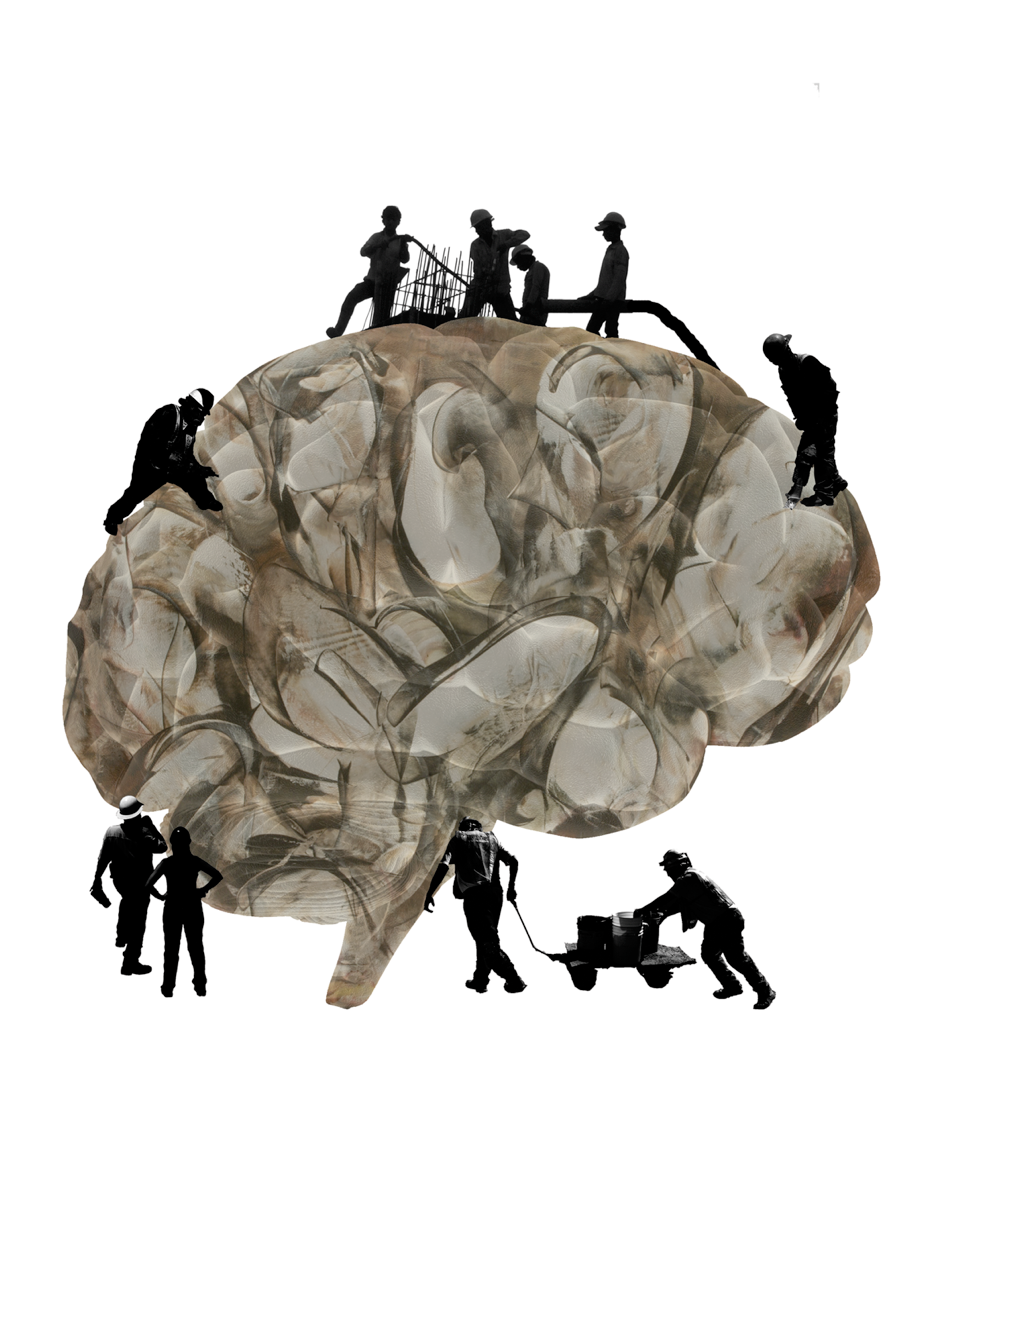
\includegraphics[height=0.75\textheight]{media/ssp/s01_i1.png}
		\end{columns}
	\end{frame}

	\begin{frame}{Spatial Semantic Pointers}
		\begin{itemize}
			\setlength{\itemsep}{0.25cm}
			\item Semantic pointers represent standard \hl{discrete} structures (lists, trees, etc.)
			\item SSPs allow recurrent convolutions to have \hl{fractional powers}
		\end{itemize}
		\begin{align*}
			B^k &= \underbrace{B \CC B \CC \ldots \CC B}_{\text{$B$ appears $k$ times}}
		\end{align*}
		\begin{itemize}
			\item Compute \hl{fractional $k$} in Fourier space
		\end{itemize}
		\begin{align*}
			B^k &= \mathcal{F}^{-1}\left\{ \mathcal{F}\{B\}^k \right\}, \quad k \in \mathbb{R} \\
			S(x, y) &= X^x \CC Y^y = \mathcal{F}^{-1}\{\mathcal{F}\{X\}^x \odot \mathcal{F}\{Y\}^y\}
		\end{align*}
	\end{frame}

	\begin{frame}{Spatial Semantic Pointers}
		\begin{columns}[c]
			\column{0.45\textwidth}
			\begin{itemize}
				\setlength{\itemsep}{0.5cm}
				\item Represent \hl{continuous space} (Clifford torus)
				\item Heat map to visualize vector contents
				\item Dot product between SSP at every possible position and $S$
			\end{itemize}
			\vspace{0.5cm}
			\begin{align*}
				\Large S(x, y) = X^x \CC Y^y
			\end{align*}
			\column{0.55\textwidth}
			\centering
			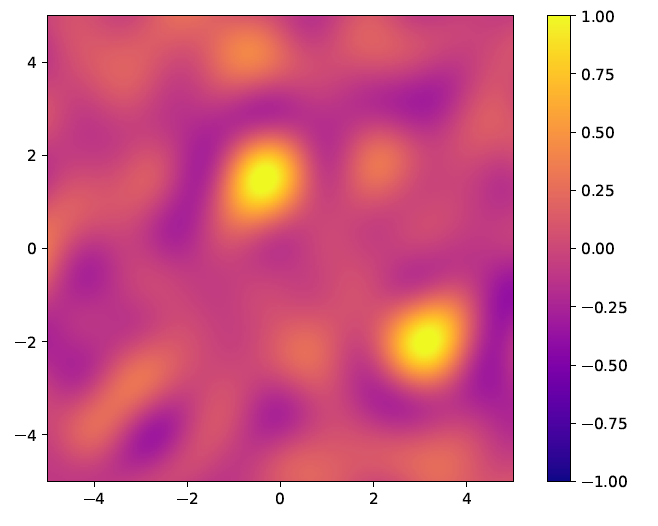
\includegraphics[height=0.85\textheight]{media/ssp/s03_i2.png}
		\end{columns}
	\end{frame}

	\begin{frame}{Mathematical Properties}
		\begin{itemize}
			\item Euclidean space is \hl{preserved} on a high-d (Clifford) torus
		\end{itemize}
		E.g.,
		\begin{align*}
			S(x_1, y_1) \CC S(x_2, y_2) &= S(x_1 + x_2, y_1 + y_2) \\
			S(x, y) \CC S(\Delta x, \Delta y) &= X^{x + \Delta x} \CC Y^{y + \Delta y}
		\end{align*}
		\begin{itemize}
			\item We get the benefits of \hl{high-d representation}, with accurate \hl{low-d Euclidean} representation
		\end{itemize}
	\end{frame}

	\begin{frame}{}
		\centering
		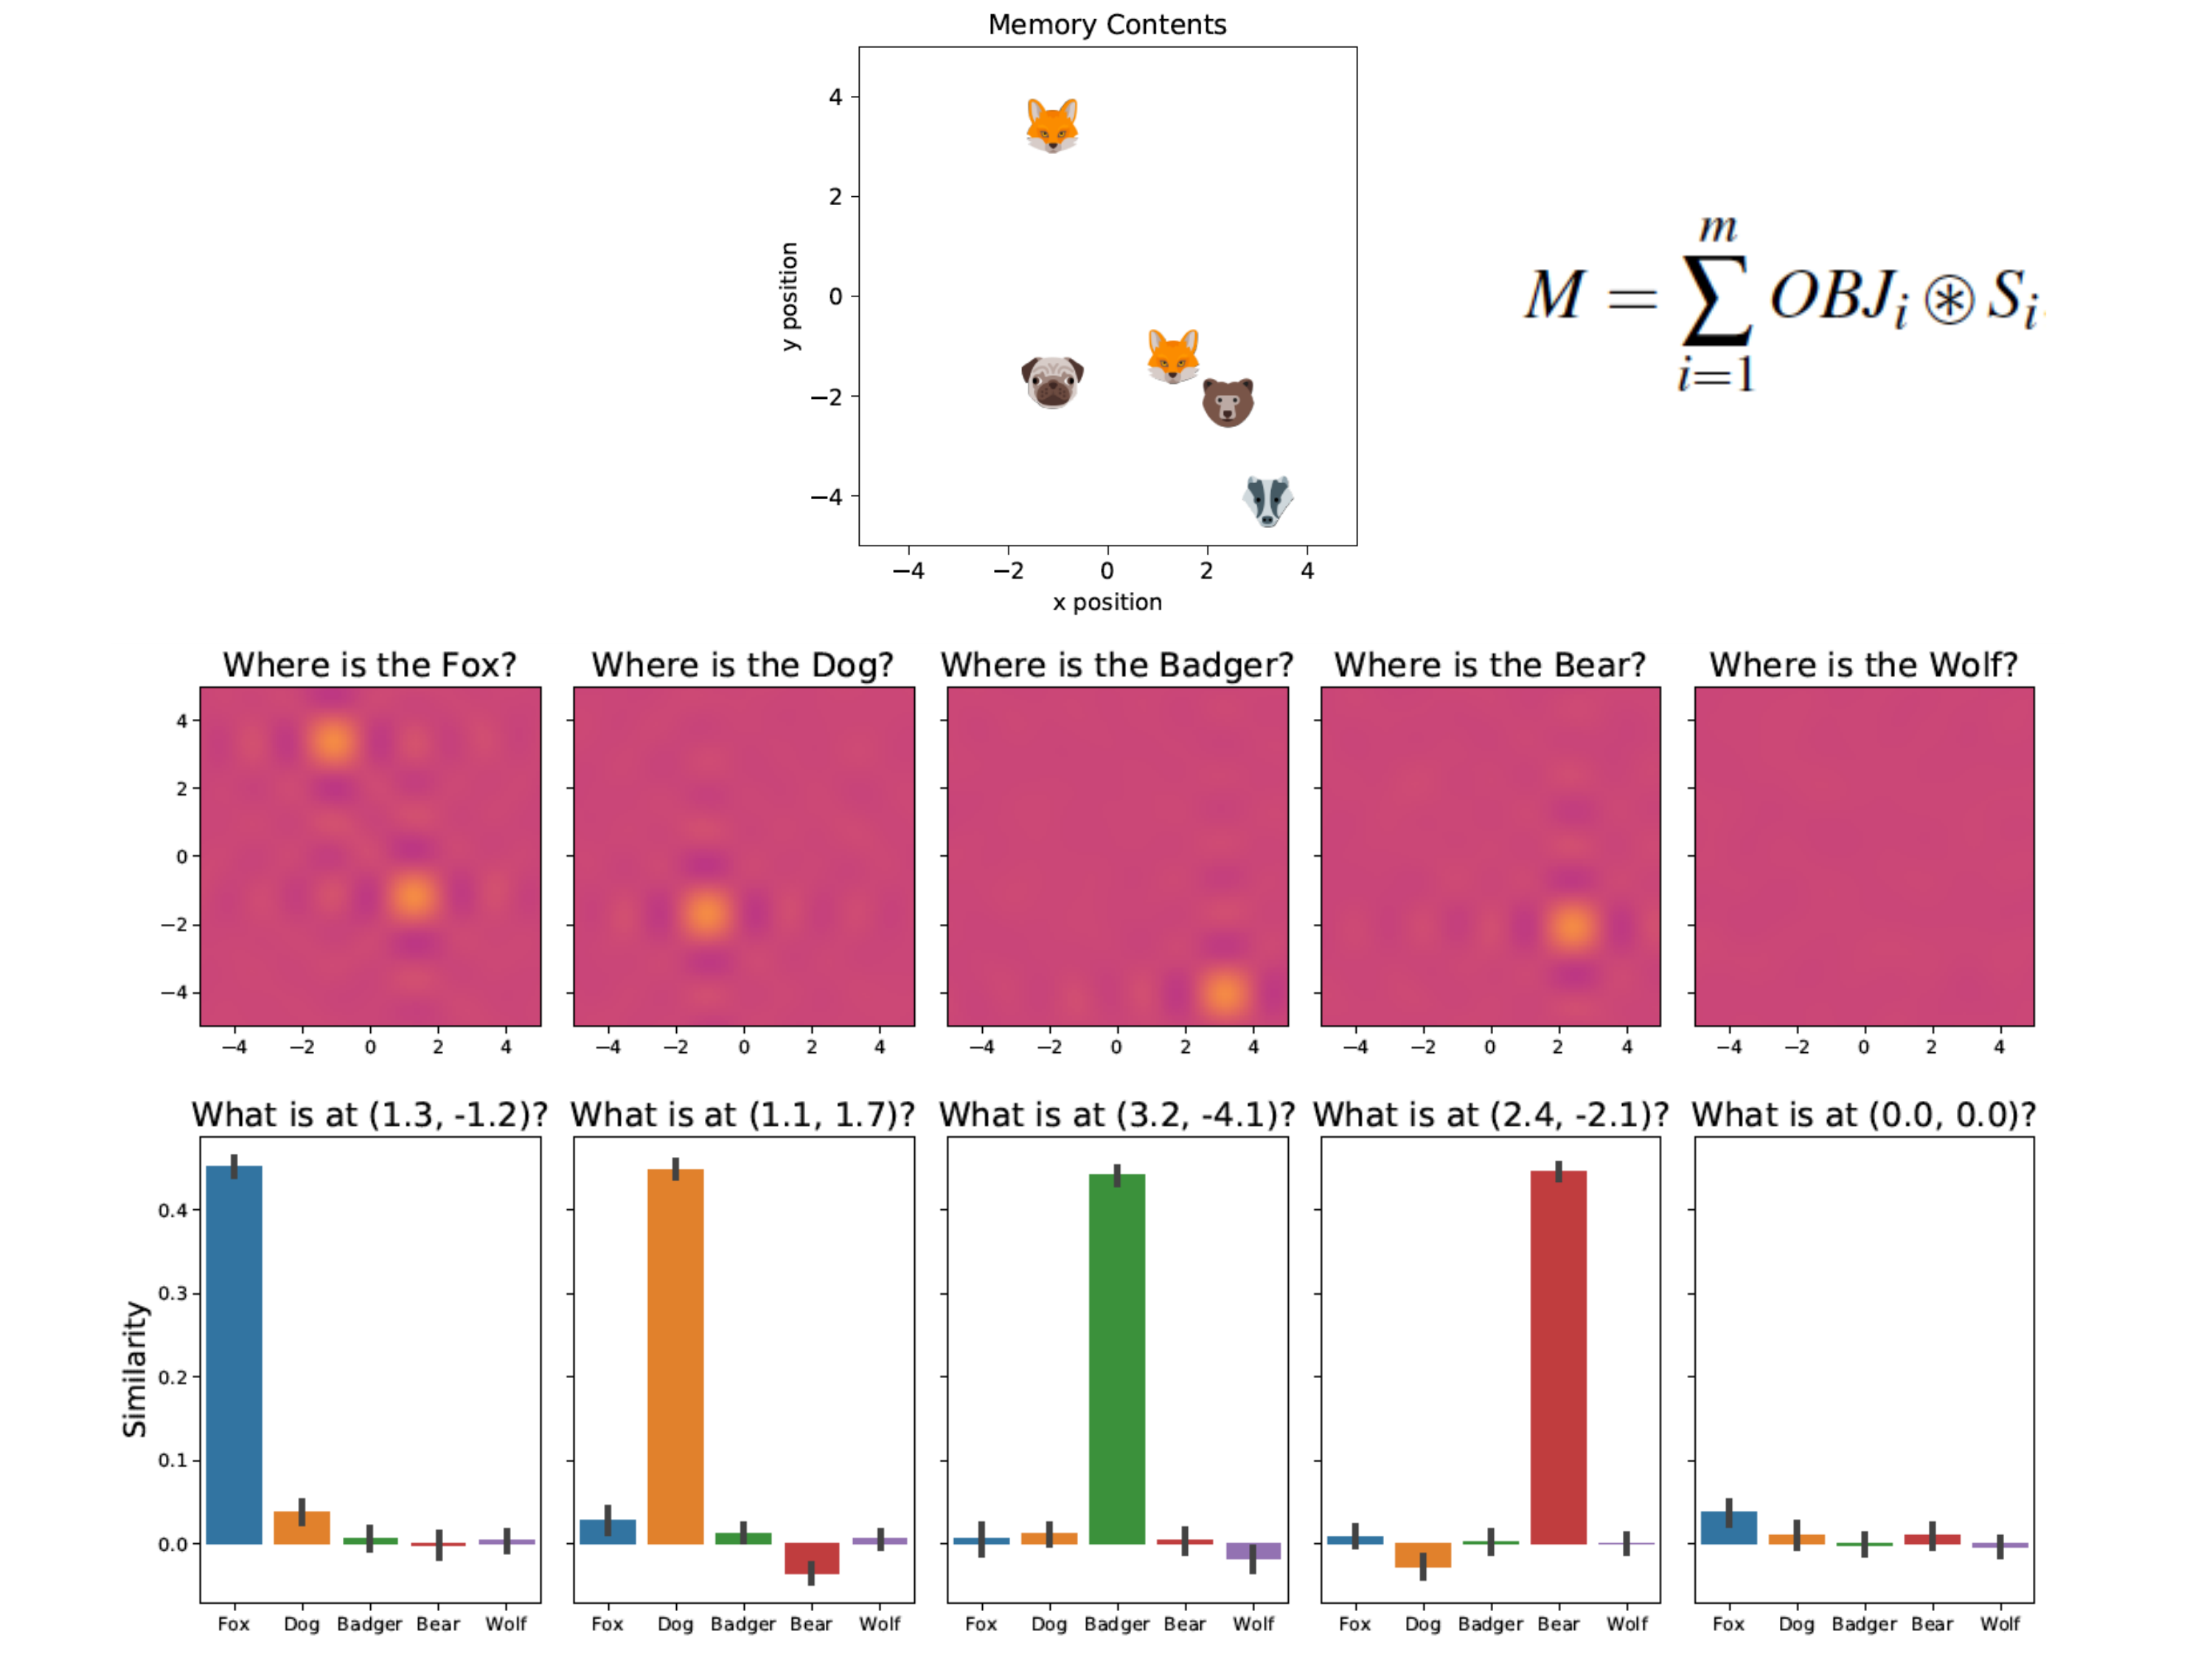
\includegraphics[height=0.95\textheight]{media/ssp/s04_full.png}
	\end{frame}

	\begin{frame}{Spatial Manipulations}
		\centering
		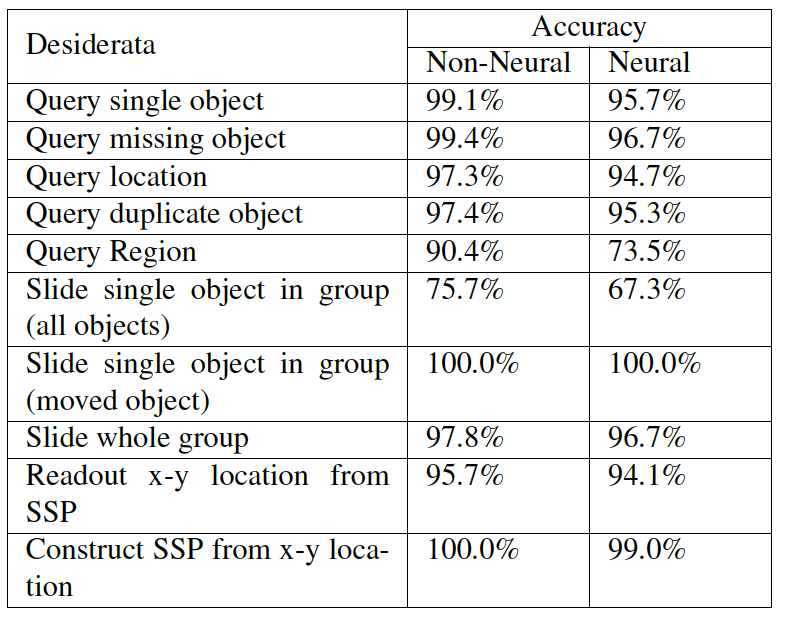
\includegraphics[height=0.85\textheight]{media/ssp/s05_i1.png}
	\end{frame}

	\begin{frame}{Navigating to Goal}
		\centering
		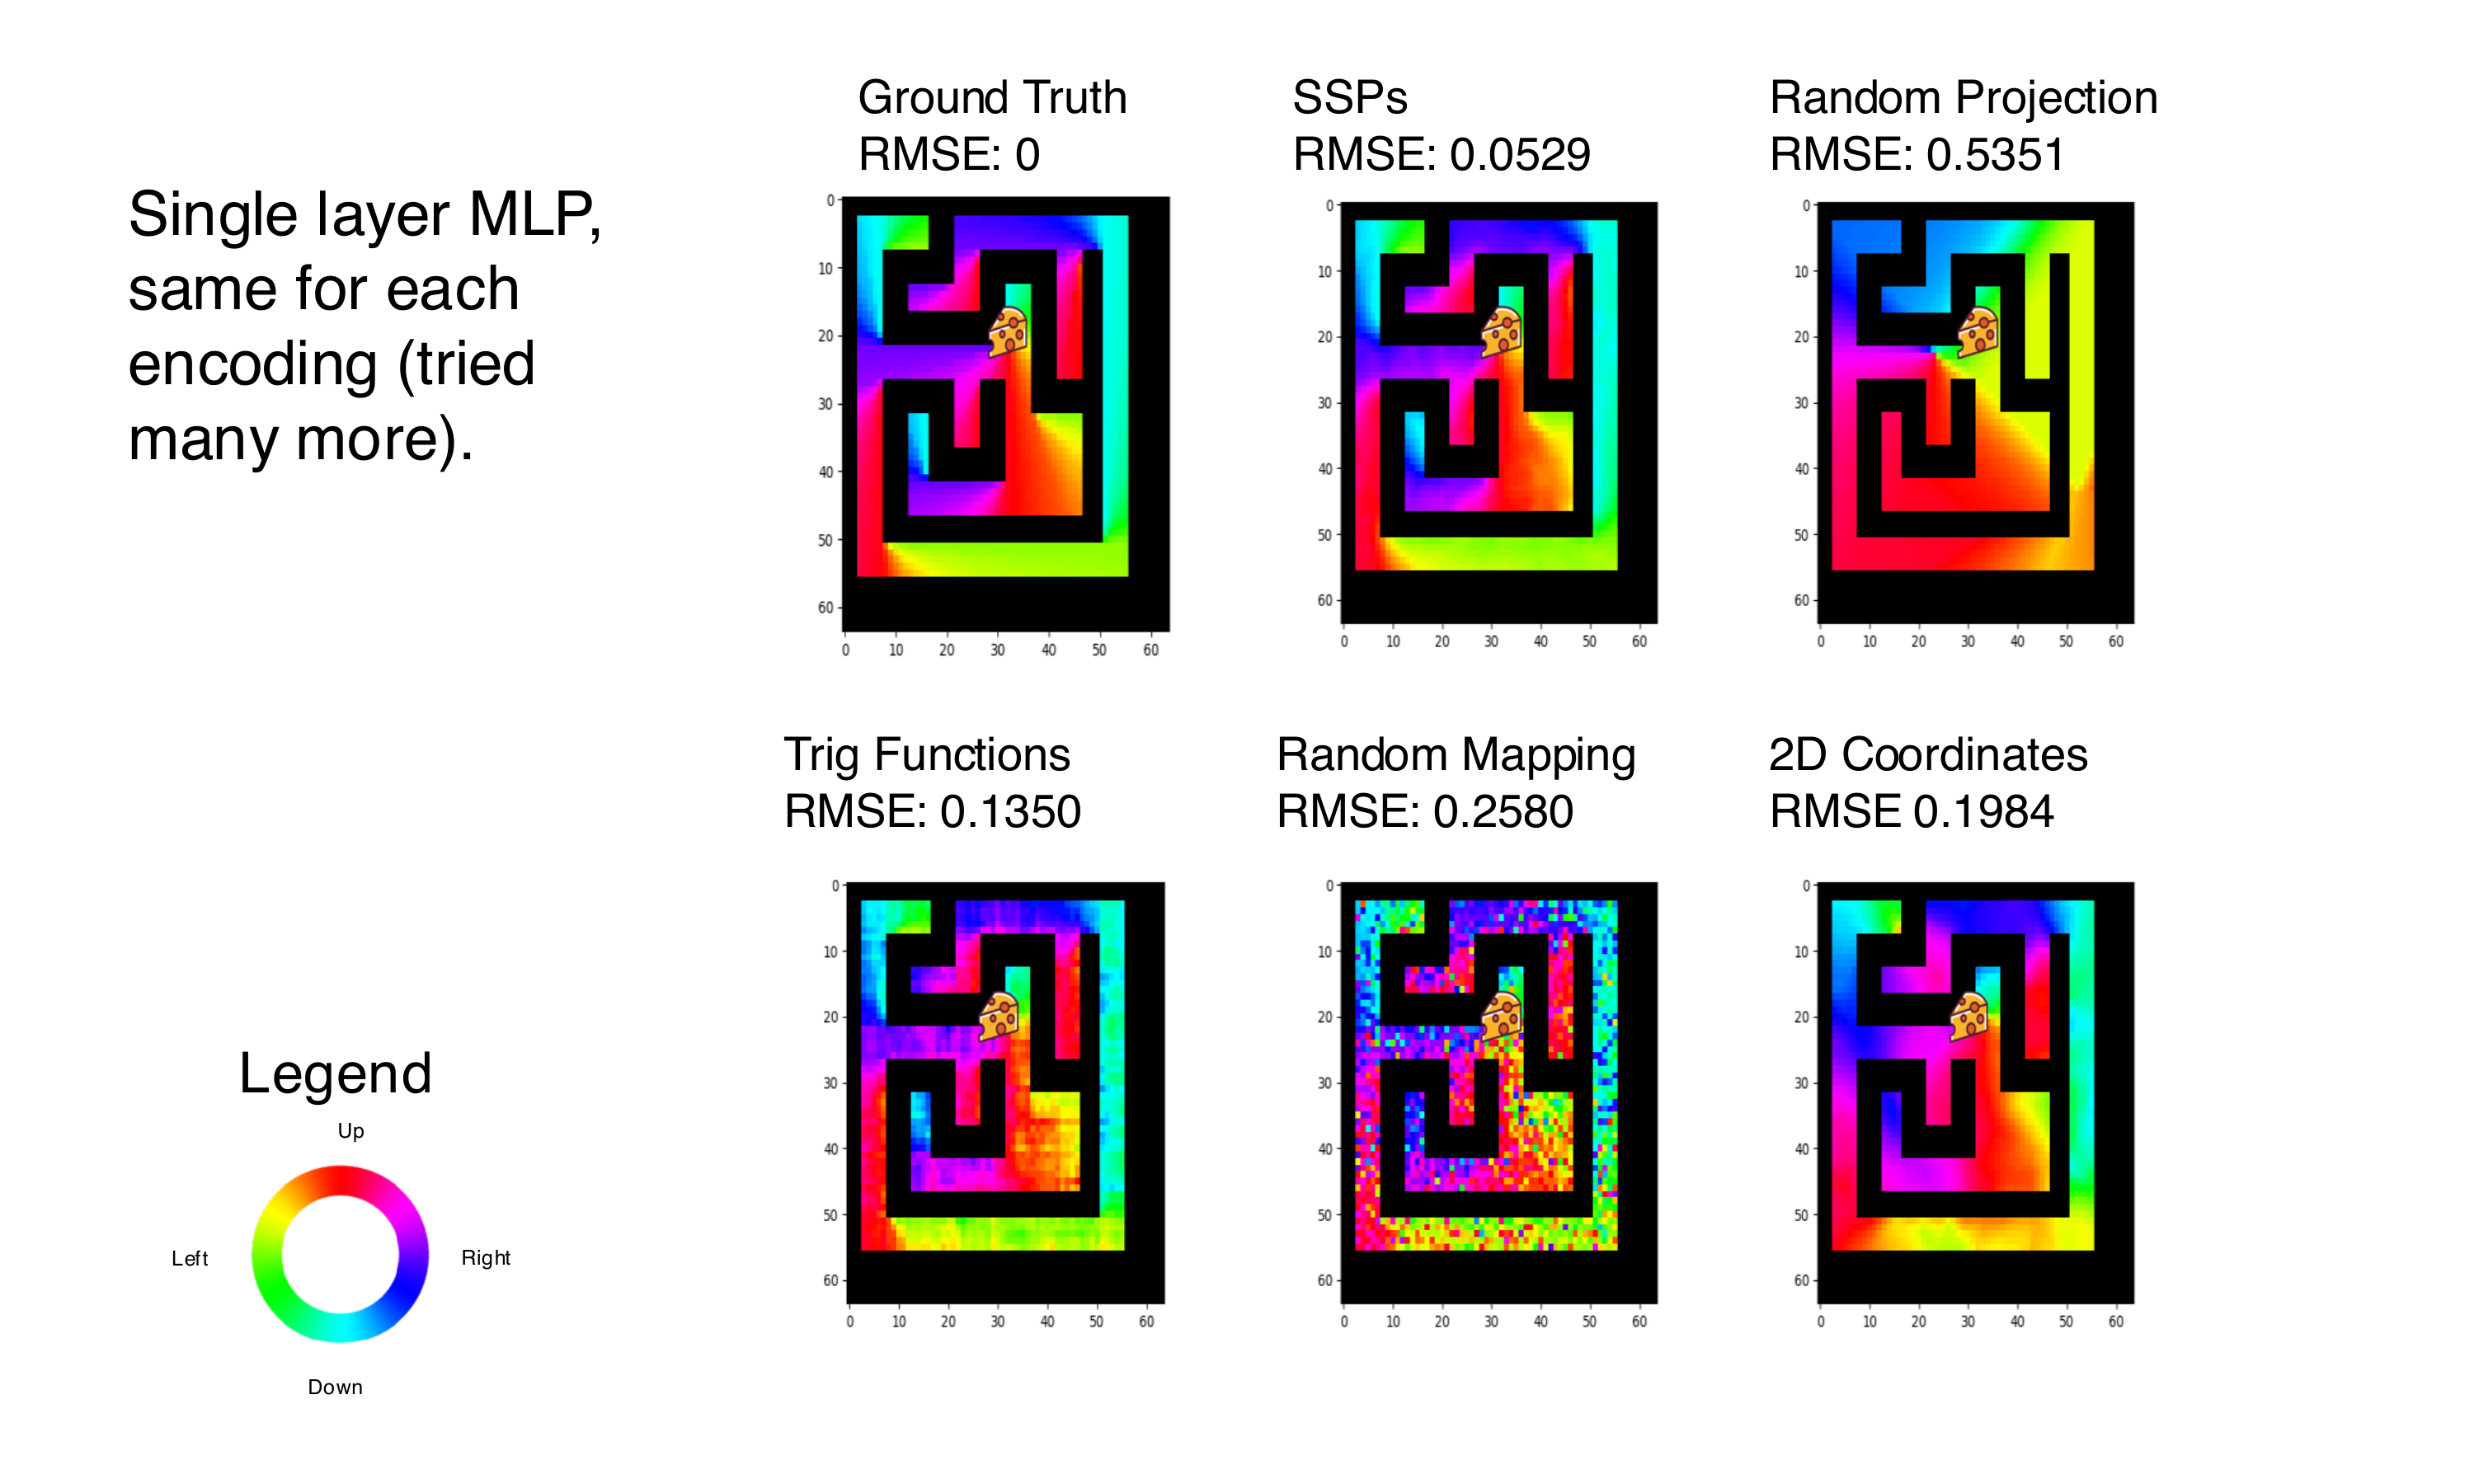
\includegraphics[height=0.85\textheight]{media/ssp/s06_body.png}
	\end{frame}

	\begin{frame}{Good for General ML}
		\centering
		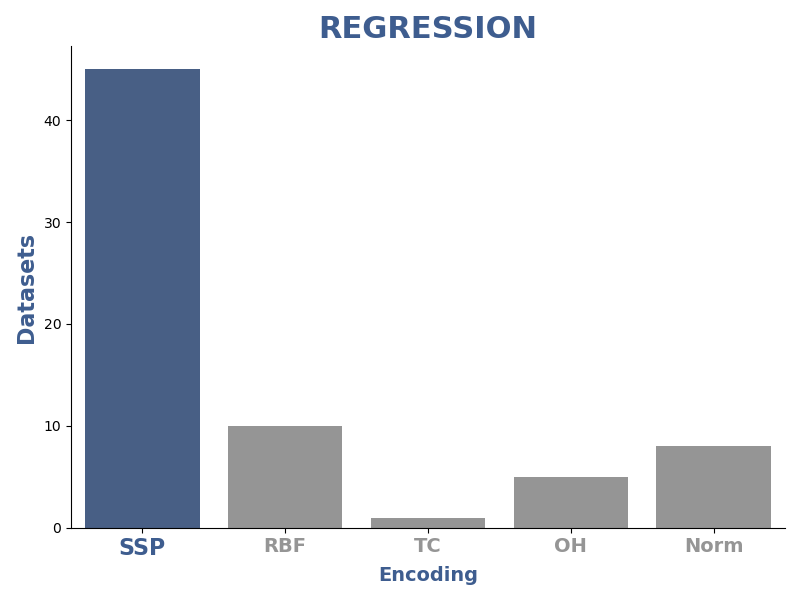
\includegraphics[width=0.48\textwidth]{media/ssp/s07_i2.png}%
		\hfill%
		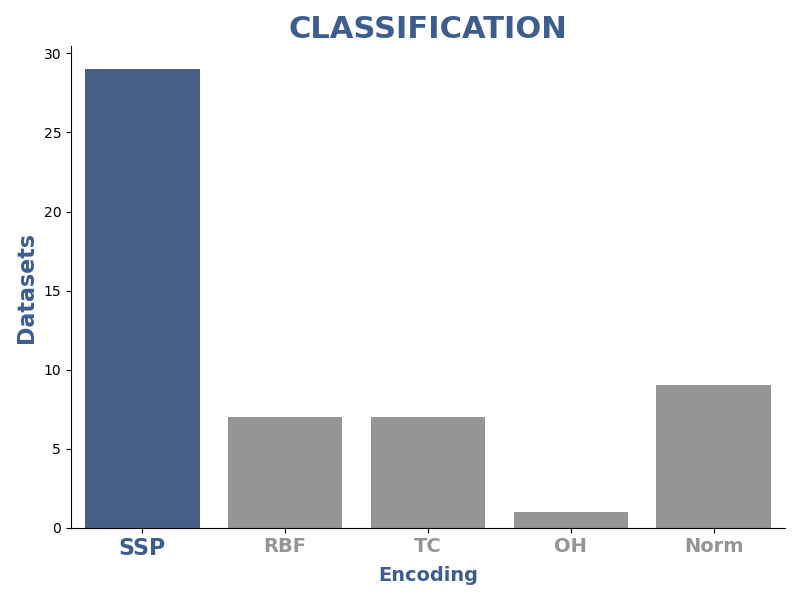
\includegraphics[width=0.48\textwidth]{media/ssp/s07_i1.png}\\[0.25cm]
		SSPs are more accurate on a large majority of 122 standard ML benchmarks.
	\end{frame}

	\begin{frame}{Scaling}
		\centering
		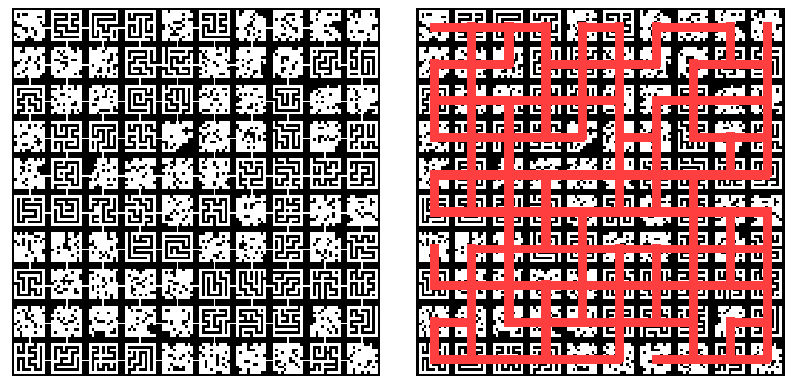
\includegraphics[width=\textwidth,height=0.78\textheight,keepaspectratio]{media/ssp/s08_i1.png}\\[0.25cm]
		Example $10 \times 10$ joined, hierarchical environment
	\end{frame}

	\begin{frame}{Scaling}
		\centering
		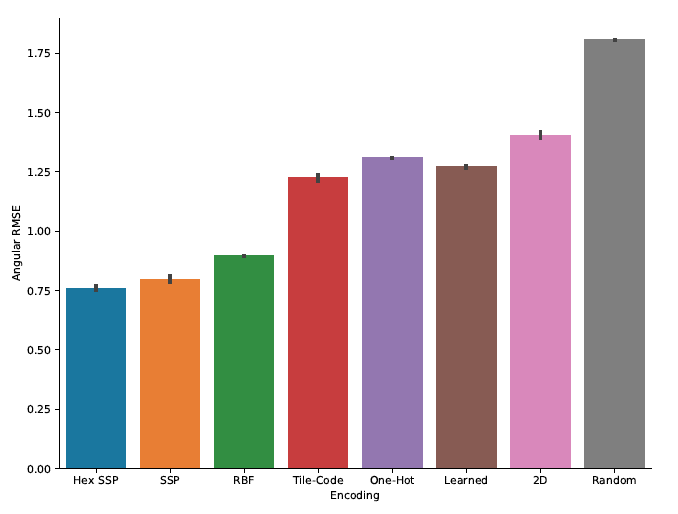
\includegraphics[height=0.78\textheight]{media/ssp/s09_i1.png}\\[0.25cm]
		Performance of different encoders on $10 \times 10$ large maze from any point to any other
	\end{frame}

	\begin{frame}{How to Choose Axis Vectors}
		\begin{itemize}
			\item Randomly (examples til now)
		\end{itemize}
		\centering
		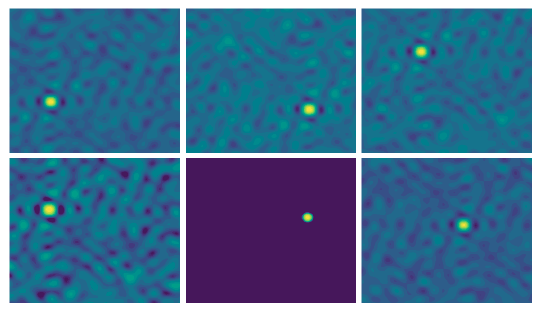
\includegraphics[height=0.68\textheight]{media/ssp/s10_i1.png}\\[0.2cm]
		Tuning curves of neurons with random axis vectors and evenly tiled SSPs as encoders
	\end{frame}

	\begin{frame}{Empirical Grid Cells}
		\centering
		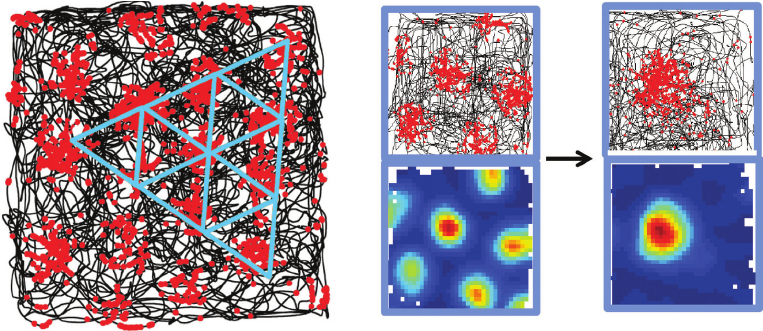
\includegraphics[width=0.95\textwidth,height=0.75\textheight,keepaspectratio]{media/ssp/s11_i1.png}\\[0.25cm]
		Grid cells in rat entorhinal cortex (Moser et al., 2015)
	\end{frame}

	\begin{frame}{How to Choose Axis Vectors}
		\begin{itemize}
			\item With plane wave structure
		\end{itemize}
		\centering
		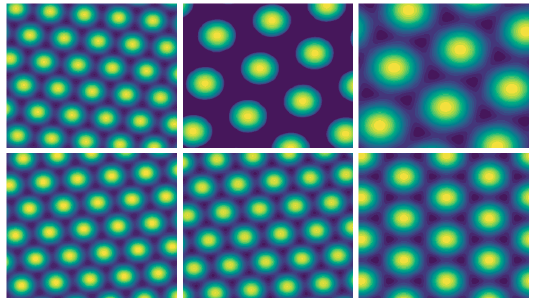
\includegraphics[height=0.65\textheight]{media/ssp/s12_i1.png}\\[0.2cm]
		Tuning curves of neurons with structured axis vectors and encoders picking out plane waves
	\end{frame}

	\begin{frame}{How to Choose Axis Vectors}
		\begin{itemize}
			\item Sums of planar waves
		\end{itemize}
		\centering
		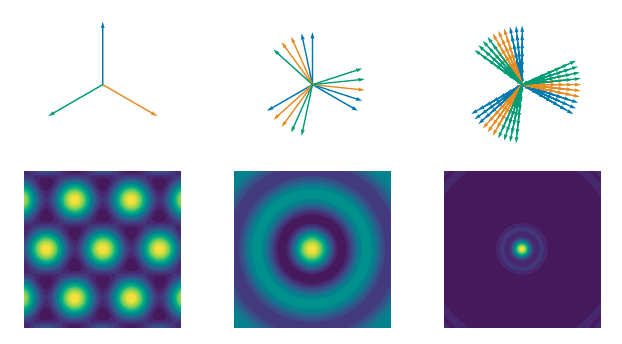
\includegraphics[width=\textwidth,height=0.75\textheight,keepaspectratio]{media/ssp/s13_i1.png}
	\end{frame}

	\begin{frame}{Grid Cells}
		\begin{itemize}
			\setlength{\itemsep}{0.25cm}
			\item With plane wave structure, spiking neurons give grid cell responses
			\item We can combine them to get \hl{place cells} (with standard NEF decoders)
		\end{itemize}
		\centering
		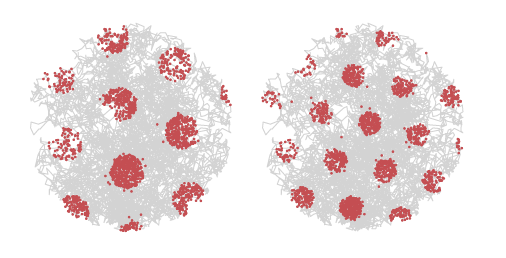
\includegraphics[height=0.55\textheight]{media/ssp/s14_i1.png}\\[0.15cm]
		SSP Grid cells
	\end{frame}

	\begin{frame}{Place Cells}
		Distance between ideal and represented place cells\\[0.25cm]
		\centering
		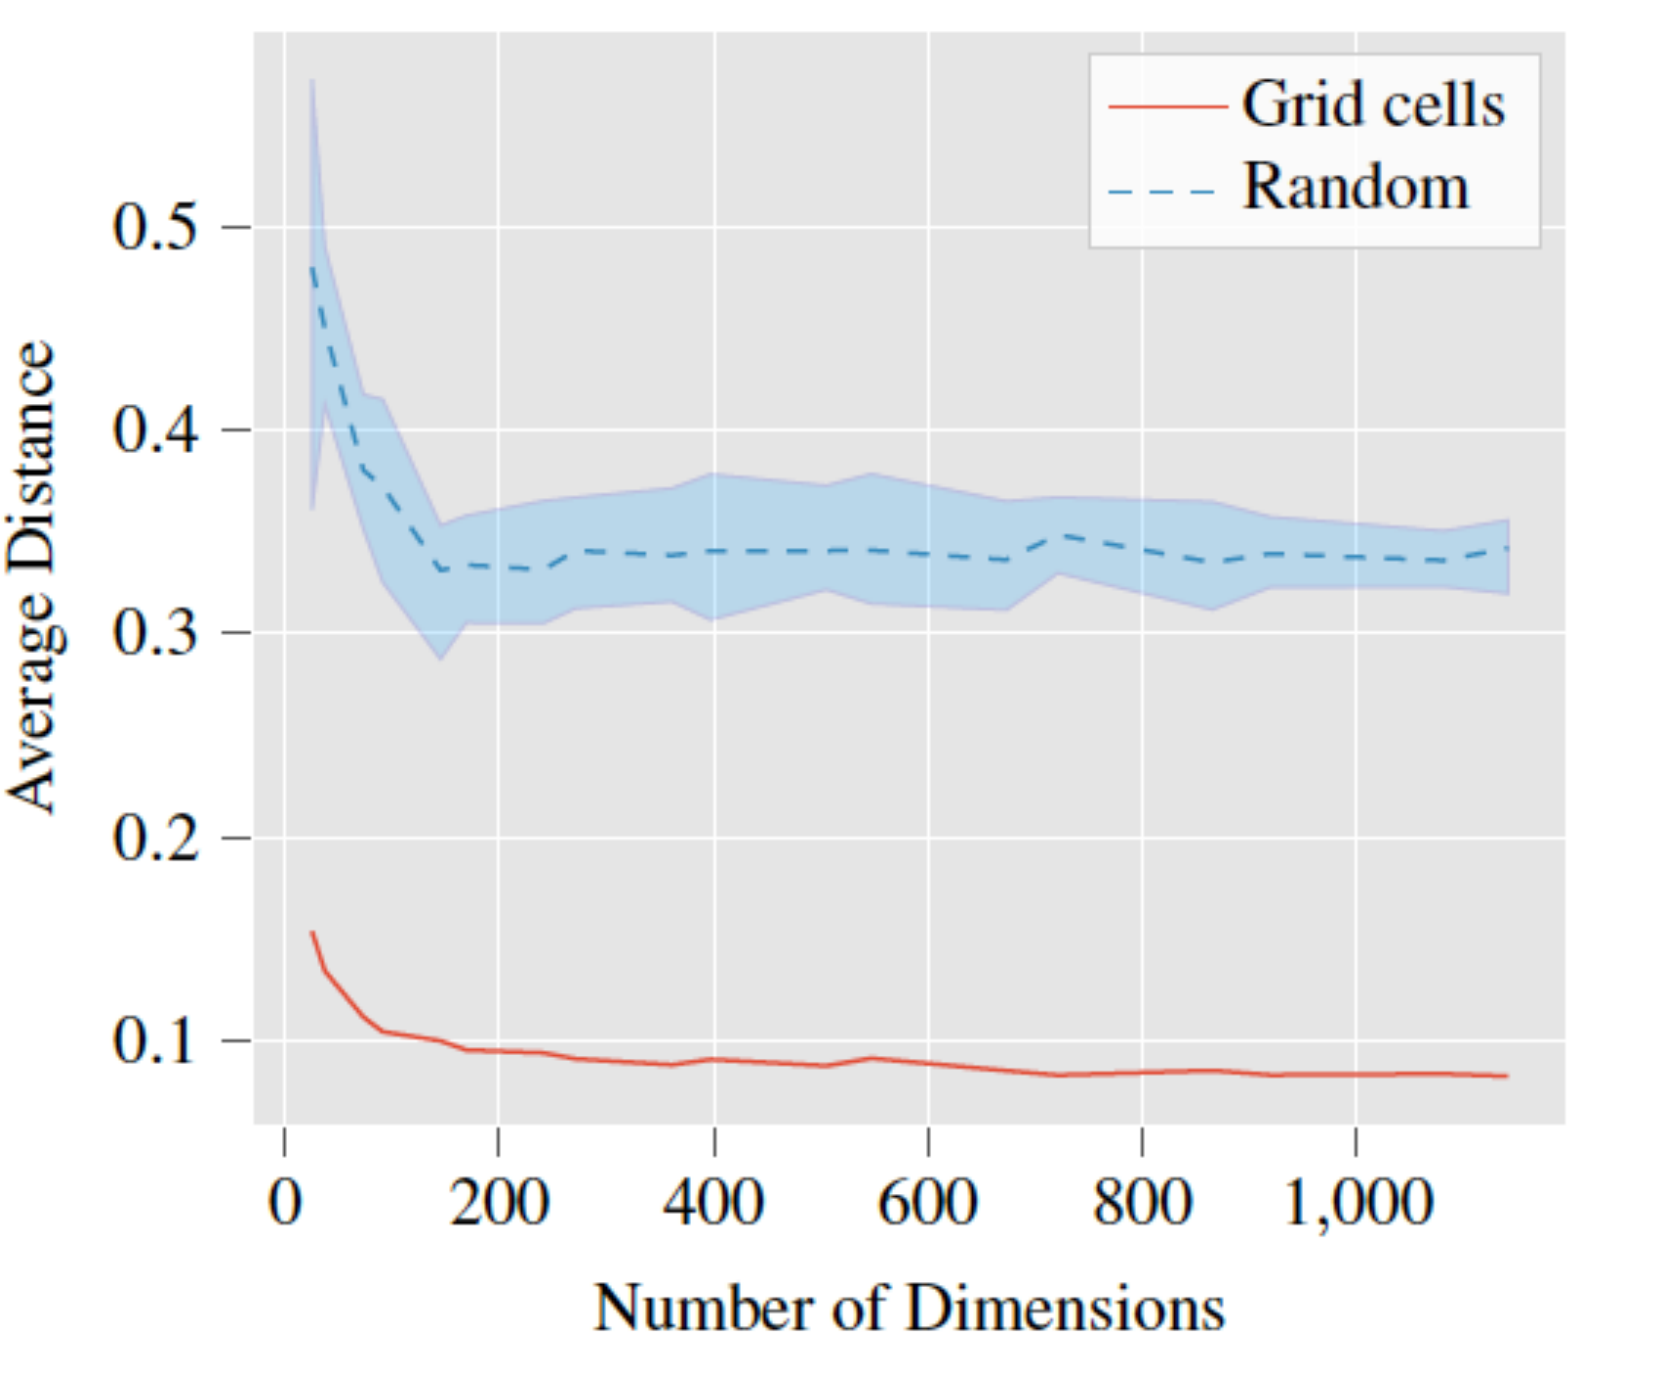
\includegraphics[height=0.72\textheight]{media/ssp/s15_a.png}%
		\hfill%
		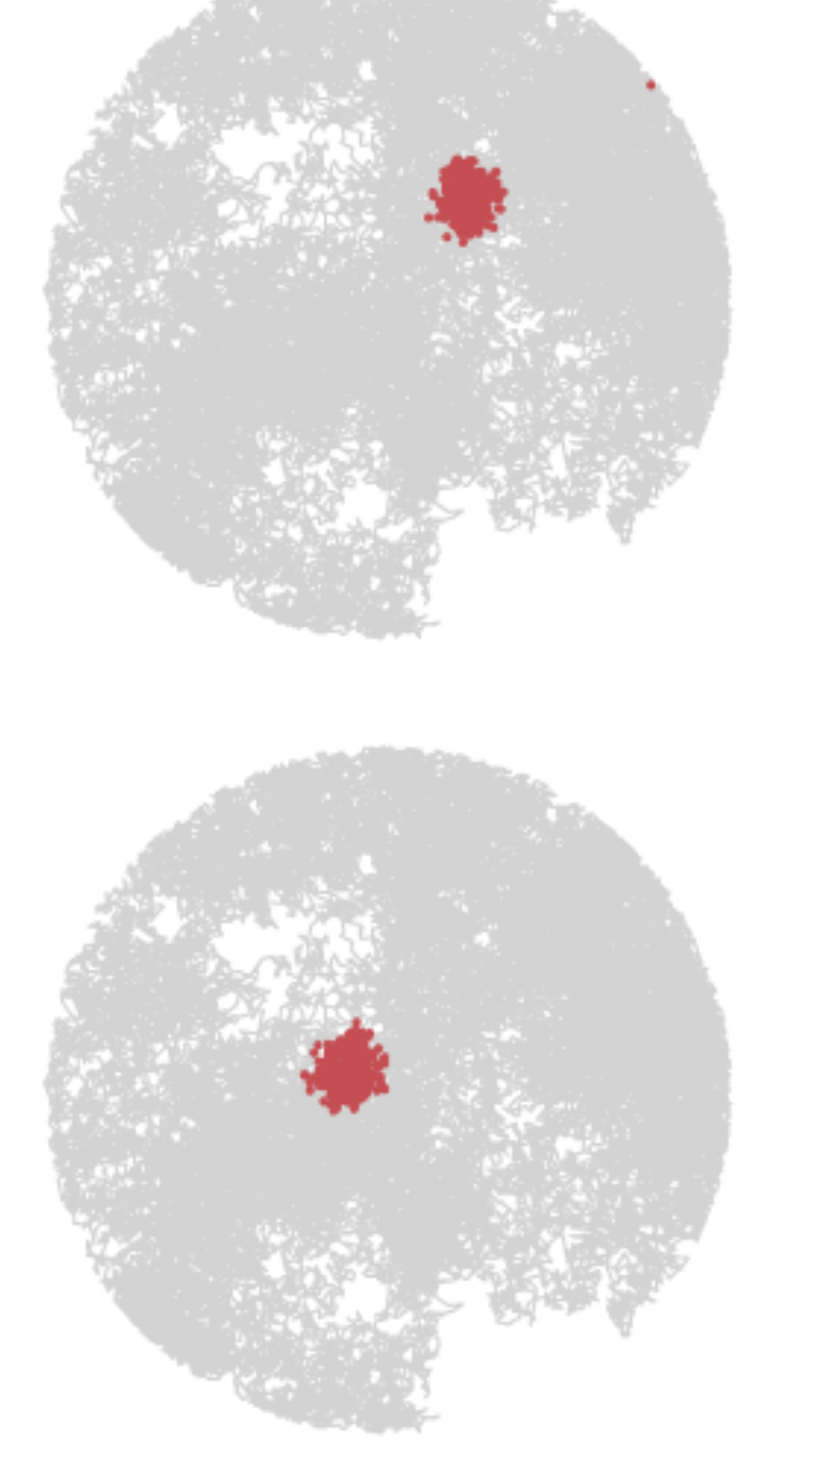
\includegraphics[height=0.76\textheight]{media/ssp/s15_b.png}
	\end{frame}

	\begin{frame}{Cognitive SLAM}
		\begin{itemize}
			\setlength{\itemsep}{0.5cm}
			\item SLAM with complex features at certain spatial locations
			\item Start with no knowledge, bind vector descriptions to particular location in space
			\item Combines spatial and `symbol' repn in neural network
			\item \hl{Semantic map} as opposed to standard `image registration' map
		\end{itemize}
	\end{frame}

	\begin{frame}{Cognitive SLAM Model}
		\centering
		\begin{columns}[c]
			\column{0.55\textwidth}
			\centering
			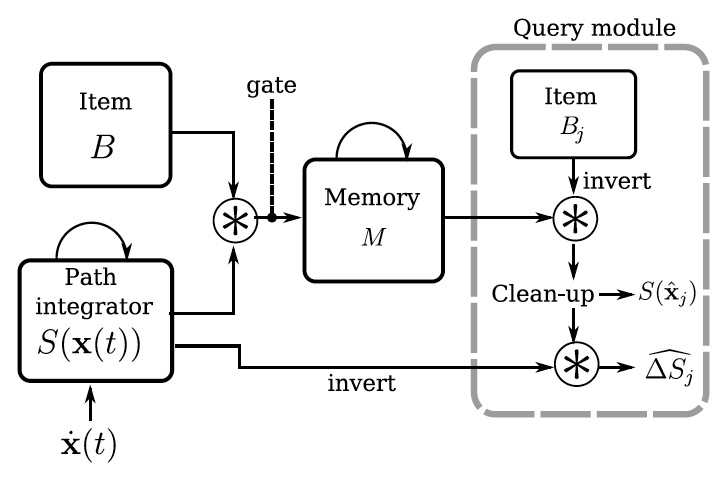
\includegraphics[width=\textwidth]{media/ssp/s17_i1.png}\\
			Full Model
			\column{0.45\textwidth}
			\centering
			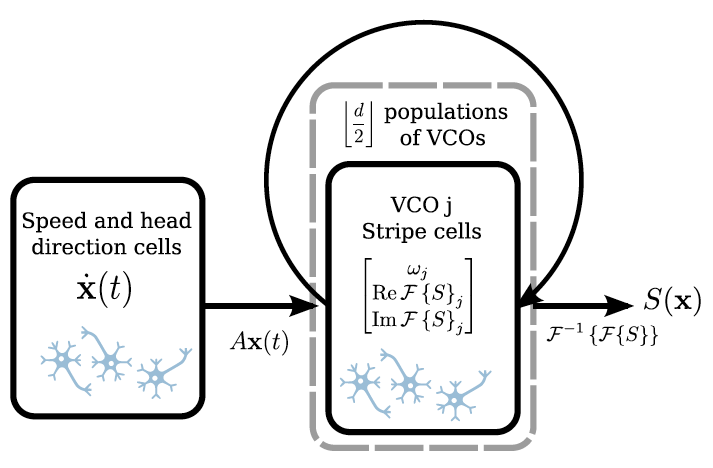
\includegraphics[width=0.95\textwidth]{media/ssp/s17_i2.png}\\
			Path Integrator
		\end{columns}
		\vspace{0.3cm}
		\begin{itemize}
			\item Path integrator tracks ego position from velocity
			\item SLAM model learns env map, outputs allo- and ego-centric position
		\end{itemize}
	\end{frame}

	\begin{frame}{Path Integration}
		\begin{itemize}
			\item One-minute long paths in 2D and 3D, spiking network
		\end{itemize}
		\centering
		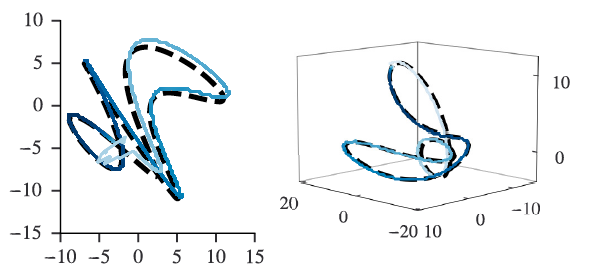
\includegraphics[width=0.9\textwidth,height=0.72\textheight,keepaspectratio]{media/ssp/s18_i1.png}
	\end{frame}

	\begin{frame}{Cognitive SLAM}
		\begin{itemize}
			\item Learns env by end of \SI{20}{\second} path, full spiking
			\item Scaling up; symbols `over' space
		\end{itemize}
		\centering
		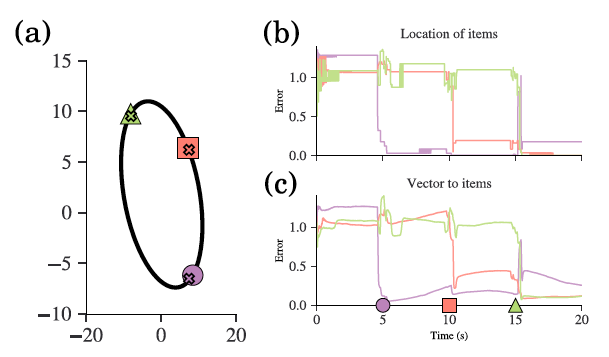
\includegraphics[height=0.68\textheight]{media/ssp/s19_i1.png}
	\end{frame}

	\begin{frame}{Cognitive SLAM}
		\begin{itemize}
			\item Learns maps in LTM bound to position
		\end{itemize}
		\centering
		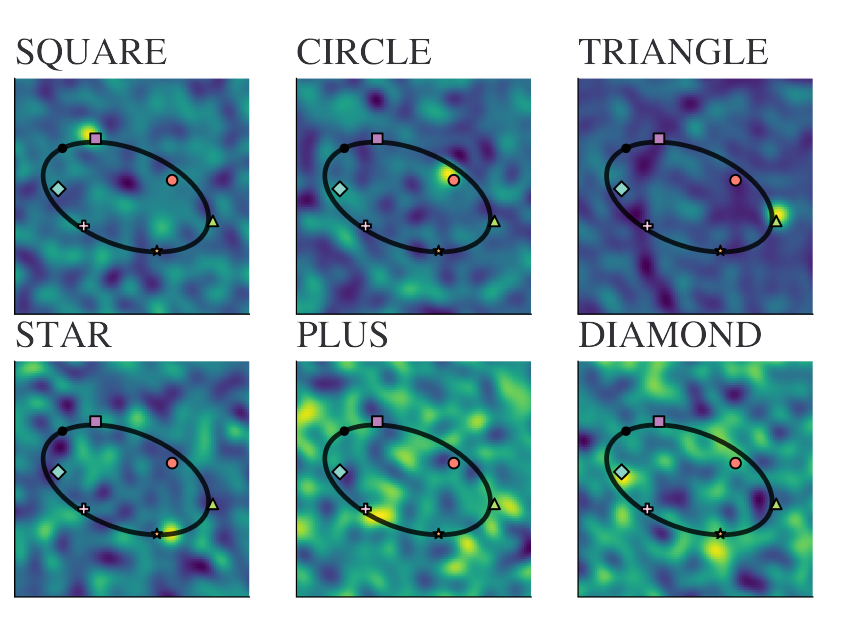
\includegraphics[height=0.72\textheight]{media/ssp/s20_i1.png}
	\end{frame}

	\begin{frame}{Navigation Network}
		Combined the above into a network to recall location and navigate to arbitrary objects in a maze.\\[0.25cm]
		\centering
		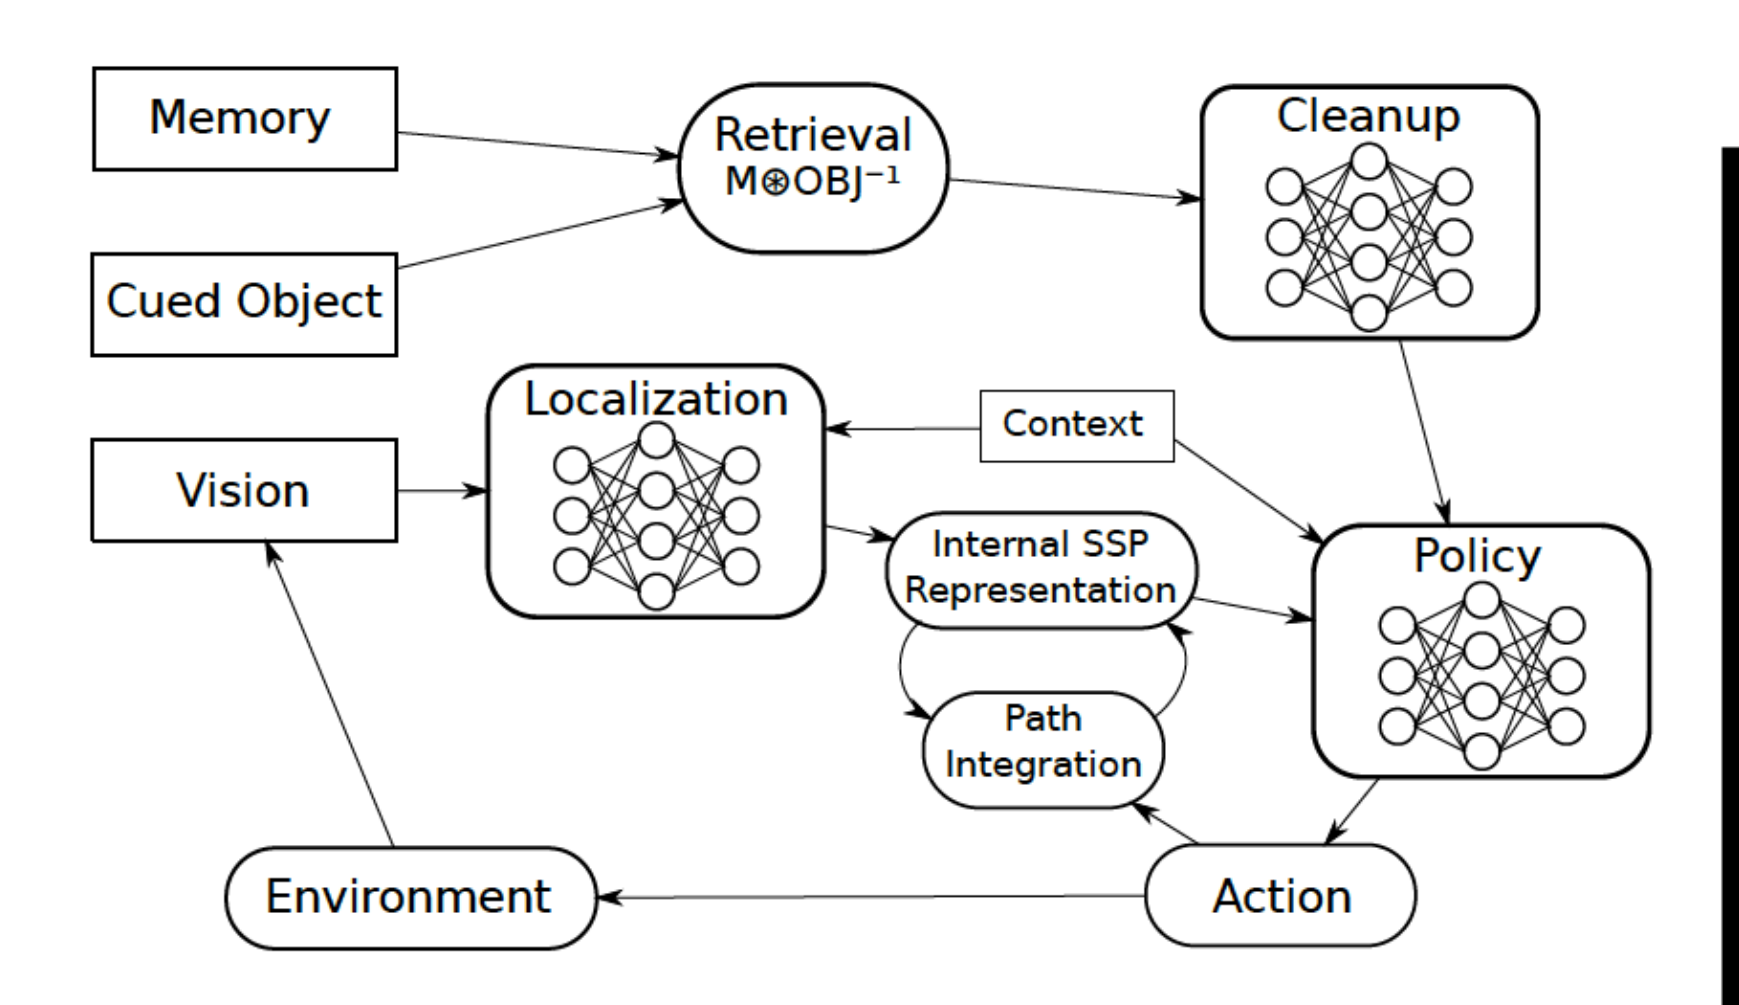
\includegraphics[width=0.52\textwidth]{media/ssp/s21_a.png}%
		\hfill%
		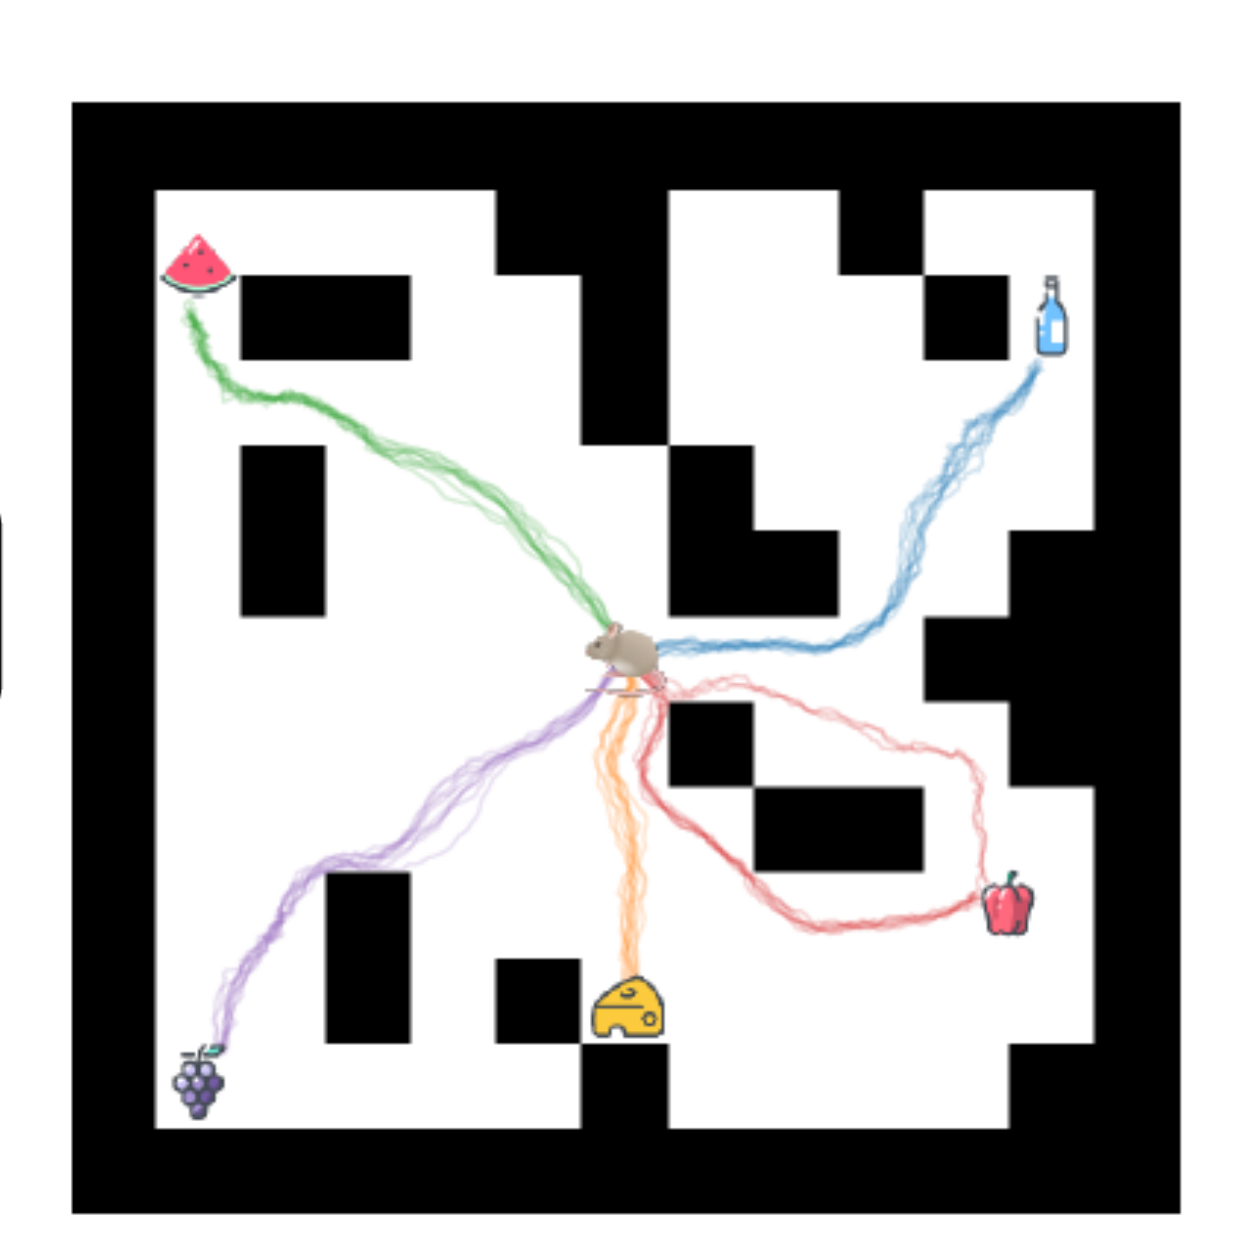
\includegraphics[height=0.62\textheight]{media/ssp/s21_b.png}
	\end{frame}

	\begin{frame}{SSPs as Probabilities}
		\begin{itemize}
			\setlength{\itemsep}{0.75cm}
			\item SSPs can be a method for \hl{encoding and processing probabilities}
			\item Method directly connects neural networks to \hl{probabilistic reasoning}
			\item SSP based methods are \hl{efficient}
		\end{itemize}
	\end{frame}

	\begin{frame}{SSPs as Probabilities}
		\begin{itemize}
			\item Background: Kernel Density Estimators
		\end{itemize}
		\vspace{0.3cm}
		\begin{columns}[c]
			\column{0.35\textwidth}
			\begin{itemize}
				\setlength{\itemsep}{1.1cm}
				\item From a dataset
				\item With a kernel function
				\item We can estimate the probability of $x$
			\end{itemize}
			\column{0.6\textwidth}
			\begin{align*}
				\mathcal{D} &= (x_1, x_2, \ldots, x_n) \\[0.5cm]
				k_h(x, x') &= k\left(\frac{\|x - x'\|}{h}\right) \\[0.5cm]
				P_\mathcal{D}(X = x) &= \frac{1}{nh} \sum_{x_i \in \mathcal{D}} k_h(x, x_i)
			\end{align*}
		\end{columns}
	\end{frame}

	\begin{frame}{SSPs as Probabilities}
		\begin{itemize}
			\item Kernel Density Estimators: examples
		\end{itemize}
		\centering
		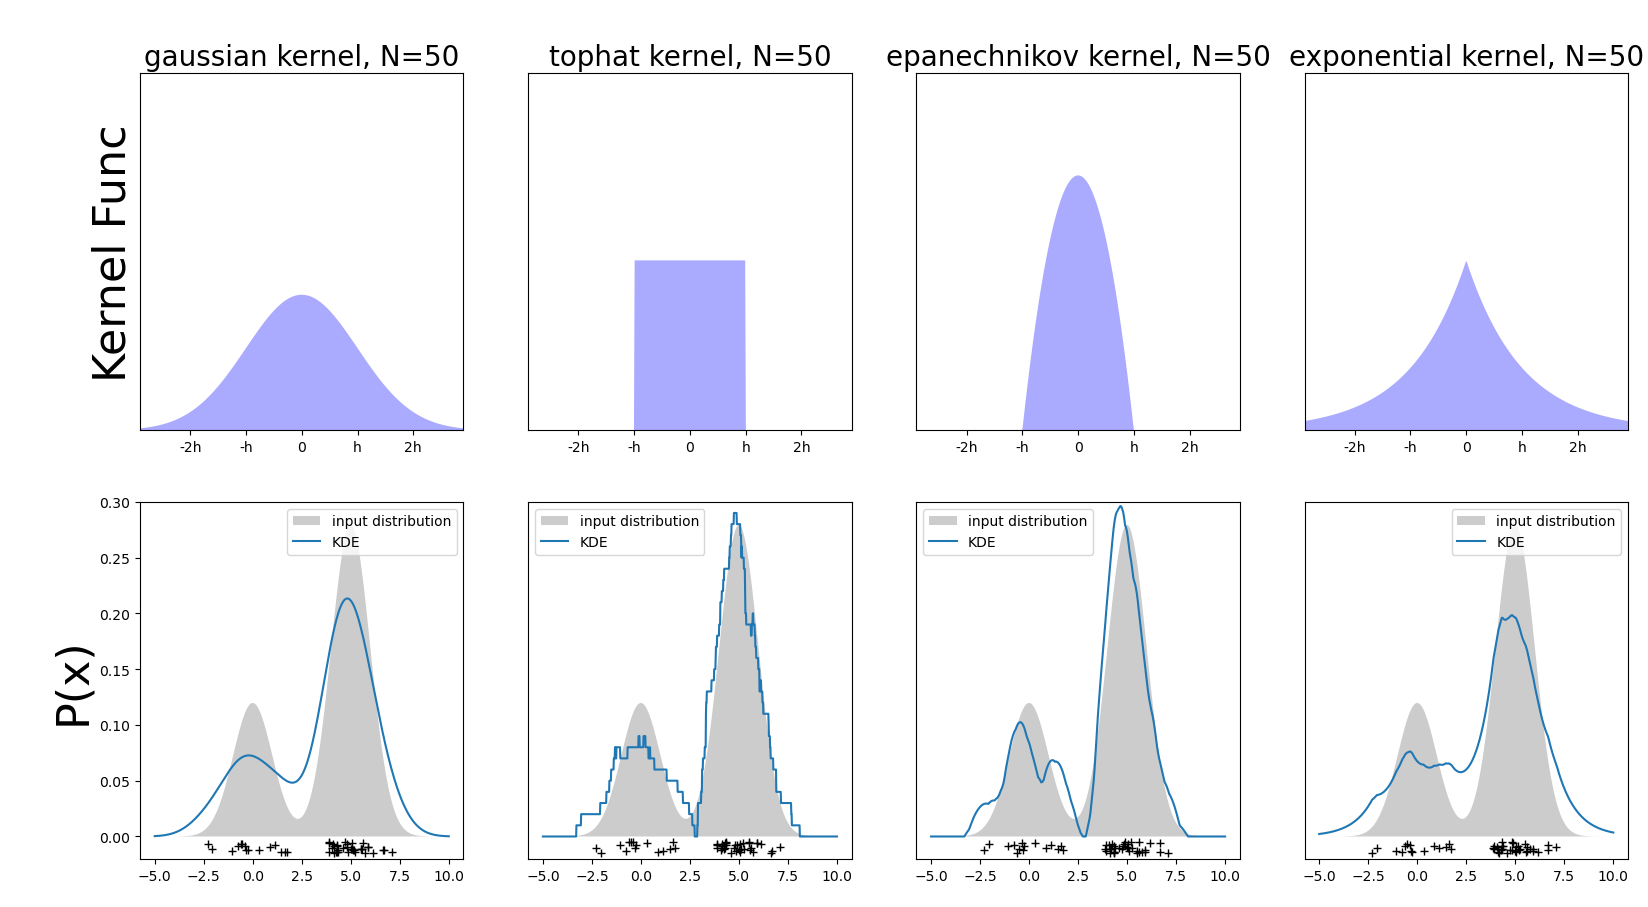
\includegraphics[width=\textwidth,height=0.75\textheight,keepaspectratio]{media/ssp/s25_i1.png}
	\end{frame}

	\begin{frame}{SSPs as Probabilities}
		\begin{itemize}
			\setlength{\itemsep}{0.25cm}
			\item Problems
			\begin{itemize}
				\item KDE memory grows linearly with the number of observations
				\item KDE time to compute a probability grows linearly with \# of observations
			\end{itemize}
			\item But\dots\ not if your kernel is a dot product
		\end{itemize}
		\vspace{0.3cm}
		\begin{align*}
			k_h(\mathbf{x}, \mathbf{x}') &\approx \phi_h(\mathbf{x}) \cdot \phi_h(\mathbf{x}') \\
			\Rightarrow \quad P(X = \mathbf{x}) &\approx \phi_h(\mathbf{x}) \cdot \sum_{\mathbf{x}_i \in \mathcal{D}} \phi_h(\mathbf{x}_i)
		\end{align*}
	\end{frame}

	\begin{frame}{SSPs as Probabilities}
		\begin{itemize}
			\item SSPs induce a quasi-kernel -- `quasi' because there are negatives
		\end{itemize}
		\centering
		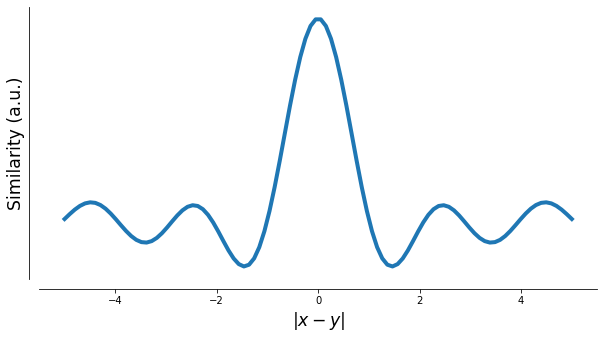
\includegraphics[height=0.58\textheight]{media/ssp/s27_i1.png}
		\begin{align*}
			\phi(\mathbf{x}) \cdot \phi(\mathbf{y}) \approx \prod_{k=1}^m \operatorname{sinc}(|x_k - y_k|)
		\end{align*}
	\end{frame}

	\begin{frame}{SSPs as Probabilities}
		\begin{itemize}
			\item Can use as a probability estimator
		\end{itemize}
		\begin{align*}
			P_\mathcal{D}(X = x) = \max\left\{0,\; \phi(x) \cdot M_{\mathcal{D},h} - \xi\right\} \quad \text{\small (Glad et al., 2003)}
		\end{align*}
		\begin{columns}[c]
			\column{0.55\textwidth}
			\centering
			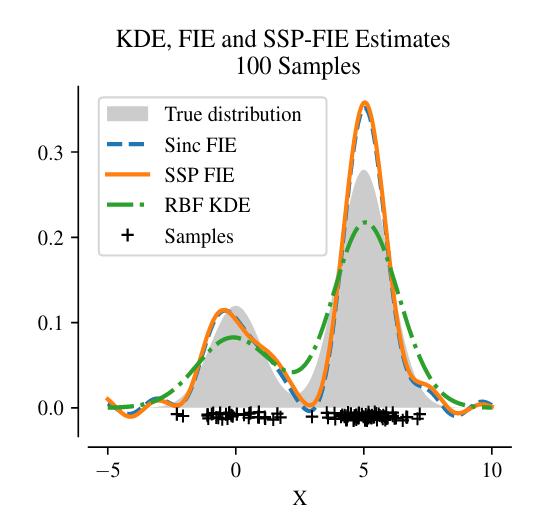
\includegraphics[width=\textwidth]{media/ssp/s28_i1.png}
			\column{0.4\textwidth}
			\centering
			\fbox{$\operatorname{ReLU}(\mathbf{w} \cdot \mathbf{z} + b)$}
		\end{columns}
	\end{frame}

	\begin{frame}{SSPs as Probabilities}
		\begin{itemize}
			\setlength{\itemsep}{0.4cm}
			\item So SSP memory is a \hl{latent probability distribution}
			\item The distribution is stored in \hl{bundles} of vector symbols
			\item We can apply manipulations to bundles to produce \hl{probabilistic statements}
		\end{itemize}
		\vspace{0.4cm}
		\begin{align*}
			M_\mathcal{D} &= \frac{1}{n} \sum_{\mathbf{x}_i \in \mathcal{D}} \phi(\mathbf{x}_i) \\
			P(\mathrm{X} = \mathbf{x}) &= \phi_h(\mathbf{x}) \cdot M_\mathcal{D}
		\end{align*}
	\end{frame}

	\begin{frame}{SSPs as Probabilities}
		\begin{itemize}
			\item Conditioning
		\end{itemize}
		\centering
		\vspace{-0.25cm}
		\begin{align*}
			P(\mathrm{X} = x \mid \mathrm{Y} = y) \approx \phi_\mathrm{X}(x) \cdot \left[ M_\mathcal{D} \CC \phi^{-1}(y) \right]
		\end{align*}
		\centering
		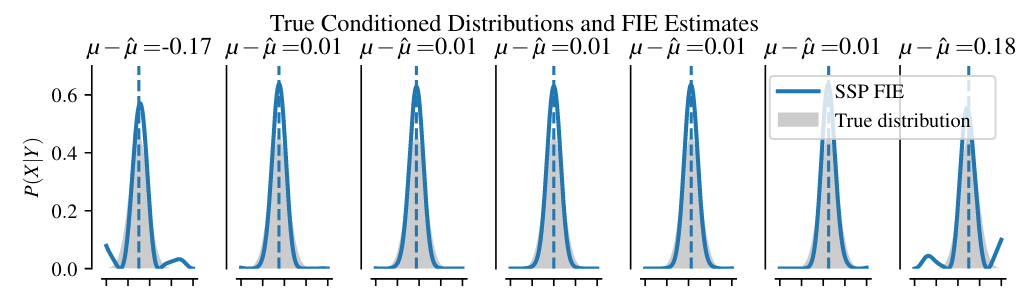
\includegraphics[width=\textwidth,height=0.6\textheight,keepaspectratio]{media/ssp/s30_i1.png}
	\end{frame}

	\begin{frame}{SSPs as Probabilities}
		\begin{columns}[c]
			\column{0.48\textwidth}
			\centering
			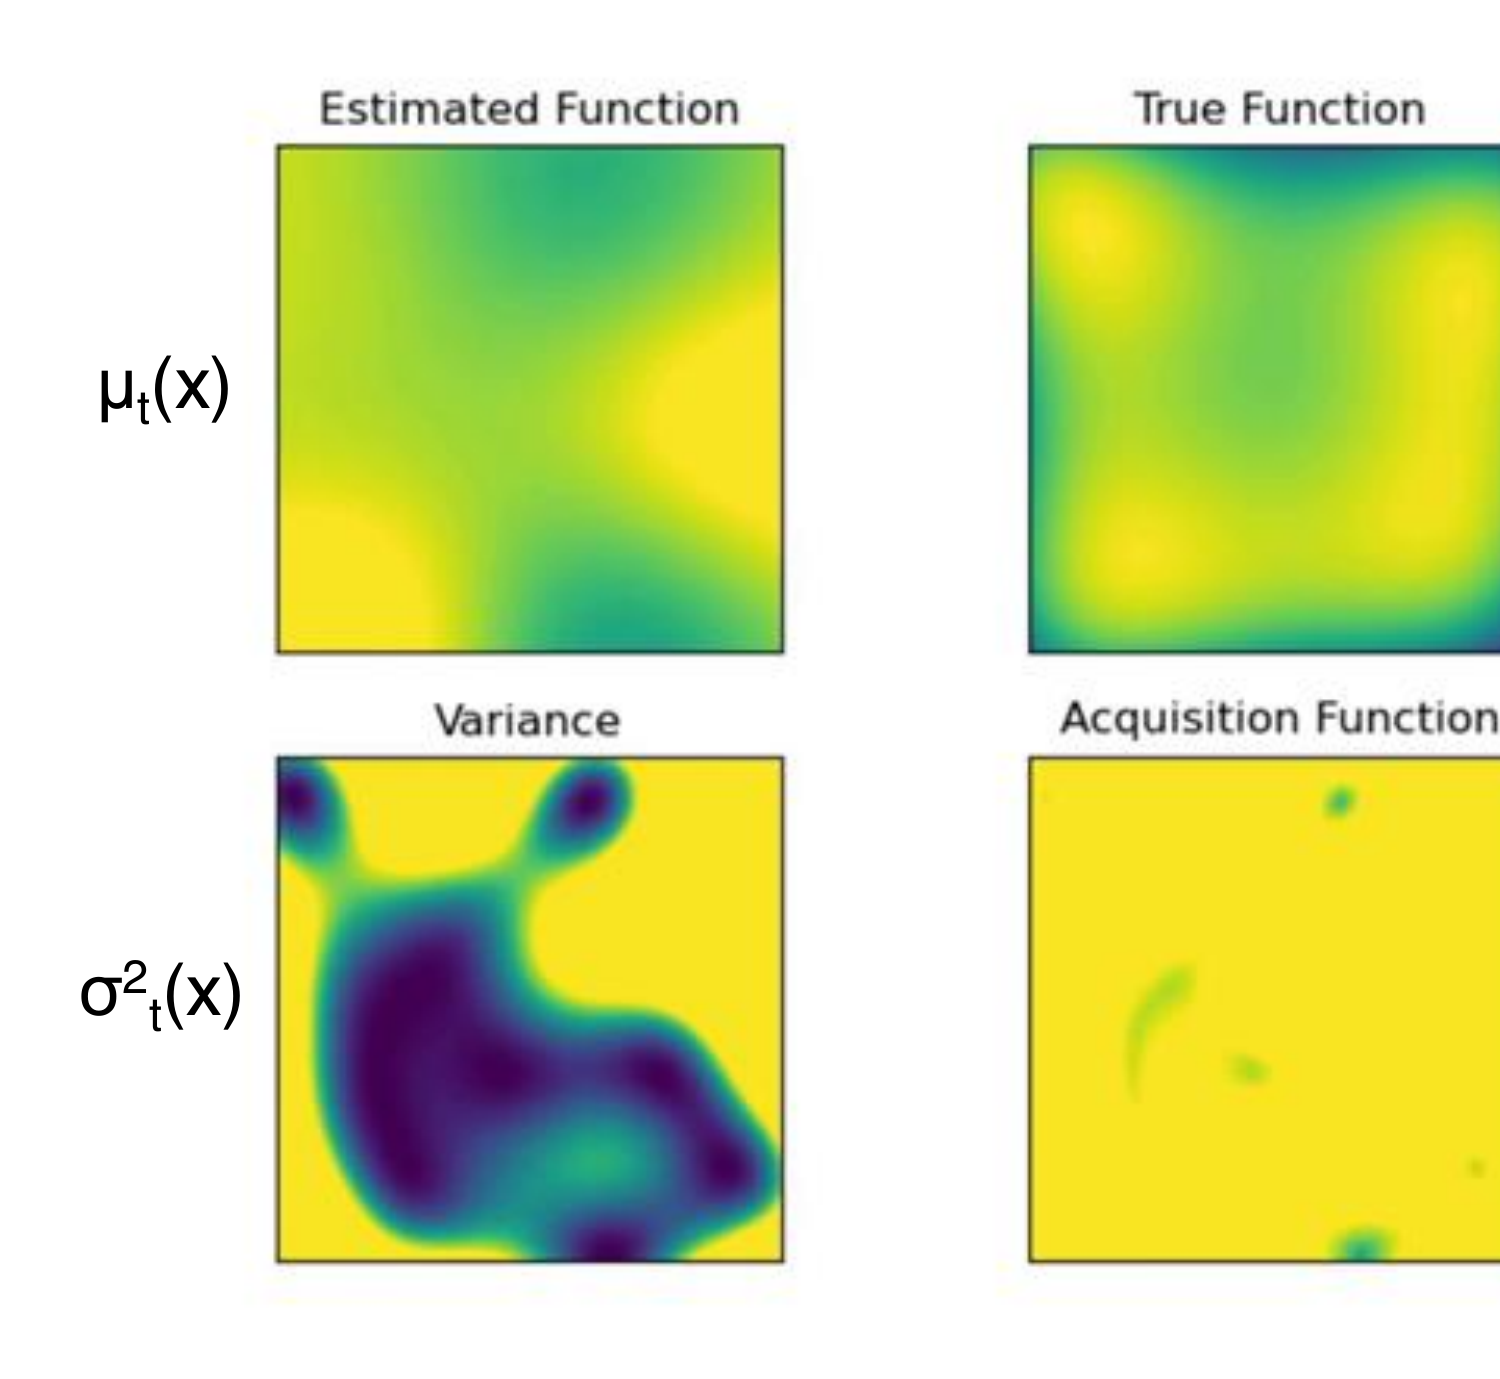
\includegraphics[width=\textwidth]{media/ssp/s31_fig.png}
			\column{0.5\textwidth}
			\begin{itemize}
				\setlength{\itemsep}{0.5cm}
				\item \hl{Mutual Information} (MI) is a common objective function used in exploration
				\item \hl{Gaussian Processes} (GPs) are a convenient, but computationally intensive tool for computing MI
				\item Can use SSPs and Bayesian linear regression to approximate a GP while improving in memory and time complexity
			\end{itemize}
		\end{columns}
	\end{frame}

	\begin{frame}{Results}
		\centering
		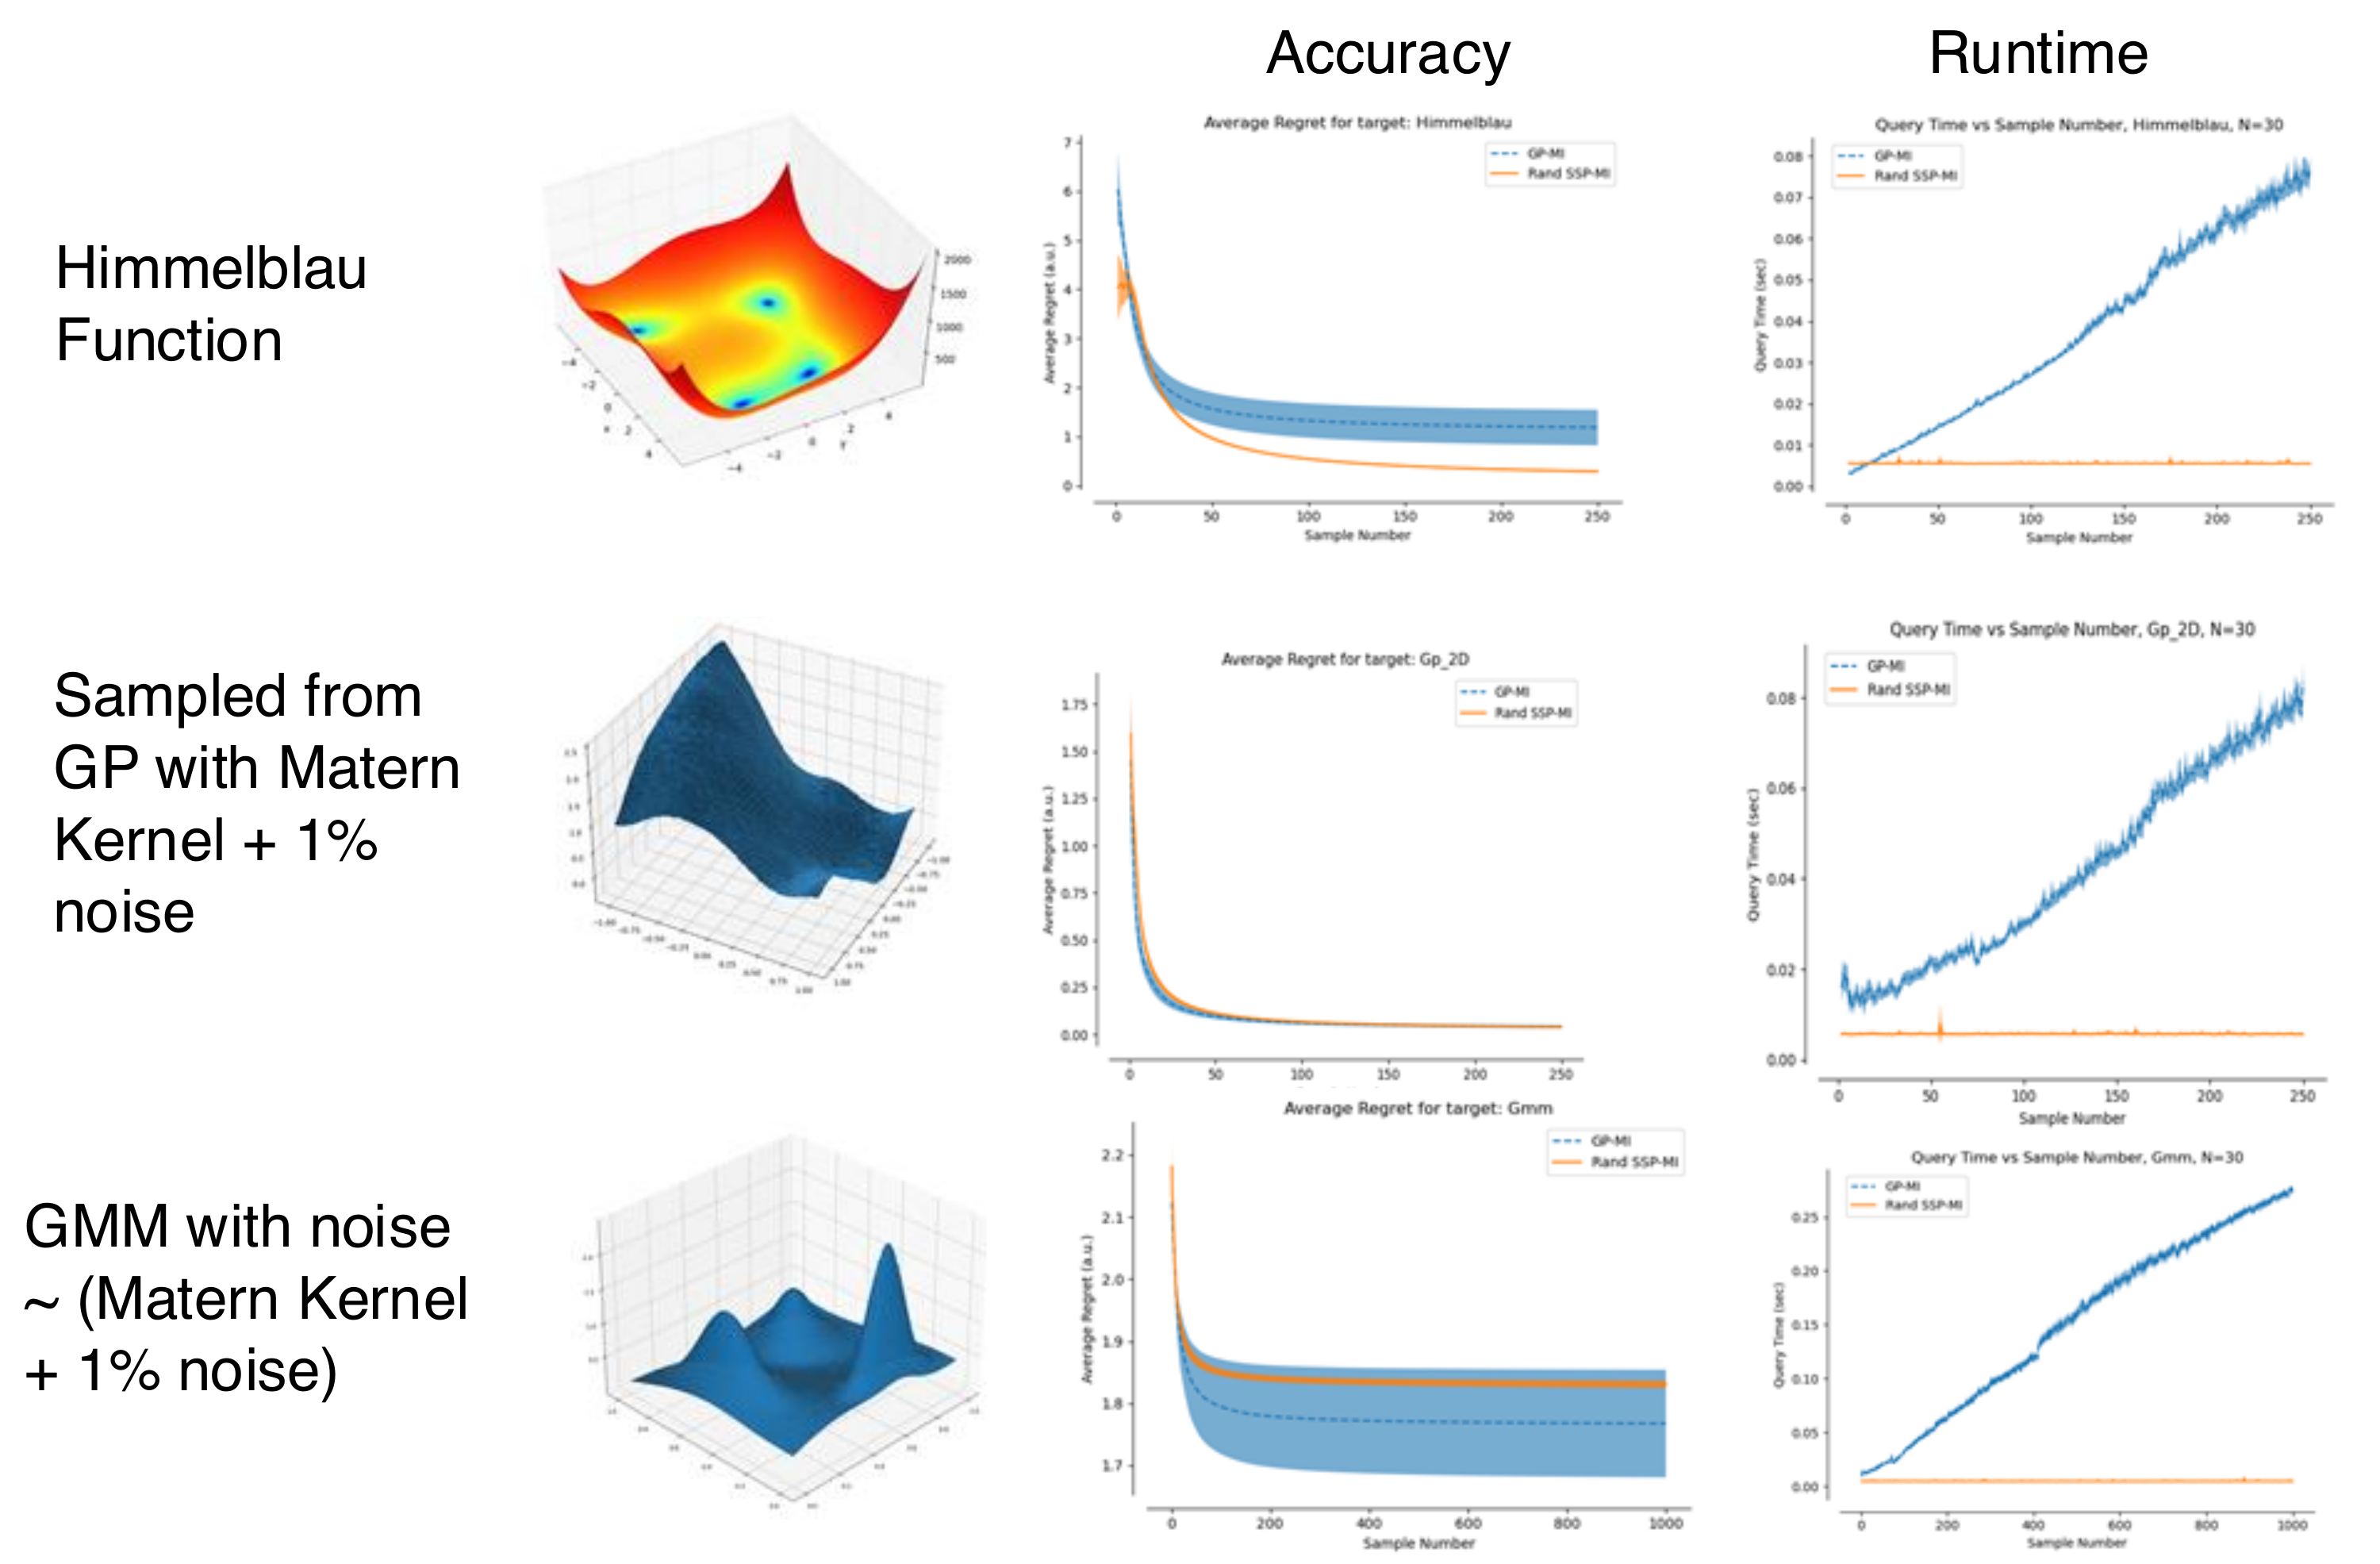
\includegraphics[width=\textwidth,height=0.88\textheight,keepaspectratio]{media/ssp/s32_body.png}
	\end{frame}

	\begin{frame}{SSPs for Sampling}
		\begin{itemize}
			\setlength{\itemsep}{0.6cm}
			\item Current methods require knowledge not accessible to a neural system (e.g., the encoding, gradients)
			\item Can use Langevin dynamics to do MCMC sampling with SSPs
			\item Supports conditioning easily as well
			\item Turns latent repns into samples in an encoding agnostic manner
		\end{itemize}
	\end{frame}

	\begin{frame}{SSPs for Sampling}
		\begin{itemize}
			\item Implementing the dynamics in a SNN generates effective samples
		\end{itemize}
		\centering
		\begin{align*}
			f(\phi(t)) = \tau\gamma \nabla_{\phi(t)} \log P(x) + \phi(t)
		\end{align*}
		\centering
		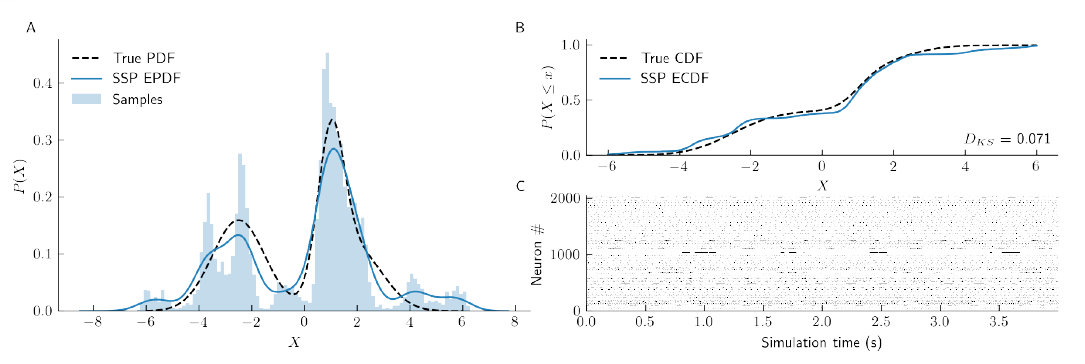
\includegraphics[width=\textwidth,height=0.6\textheight,keepaspectratio]{media/ssp/s34_i1.png}
	\end{frame}

	\begin{frame}{SSPs for Sampling}
		\begin{itemize}
			\item Sampling using dynamics for both continuous and discrete PDFs
		\end{itemize}
		\centering
		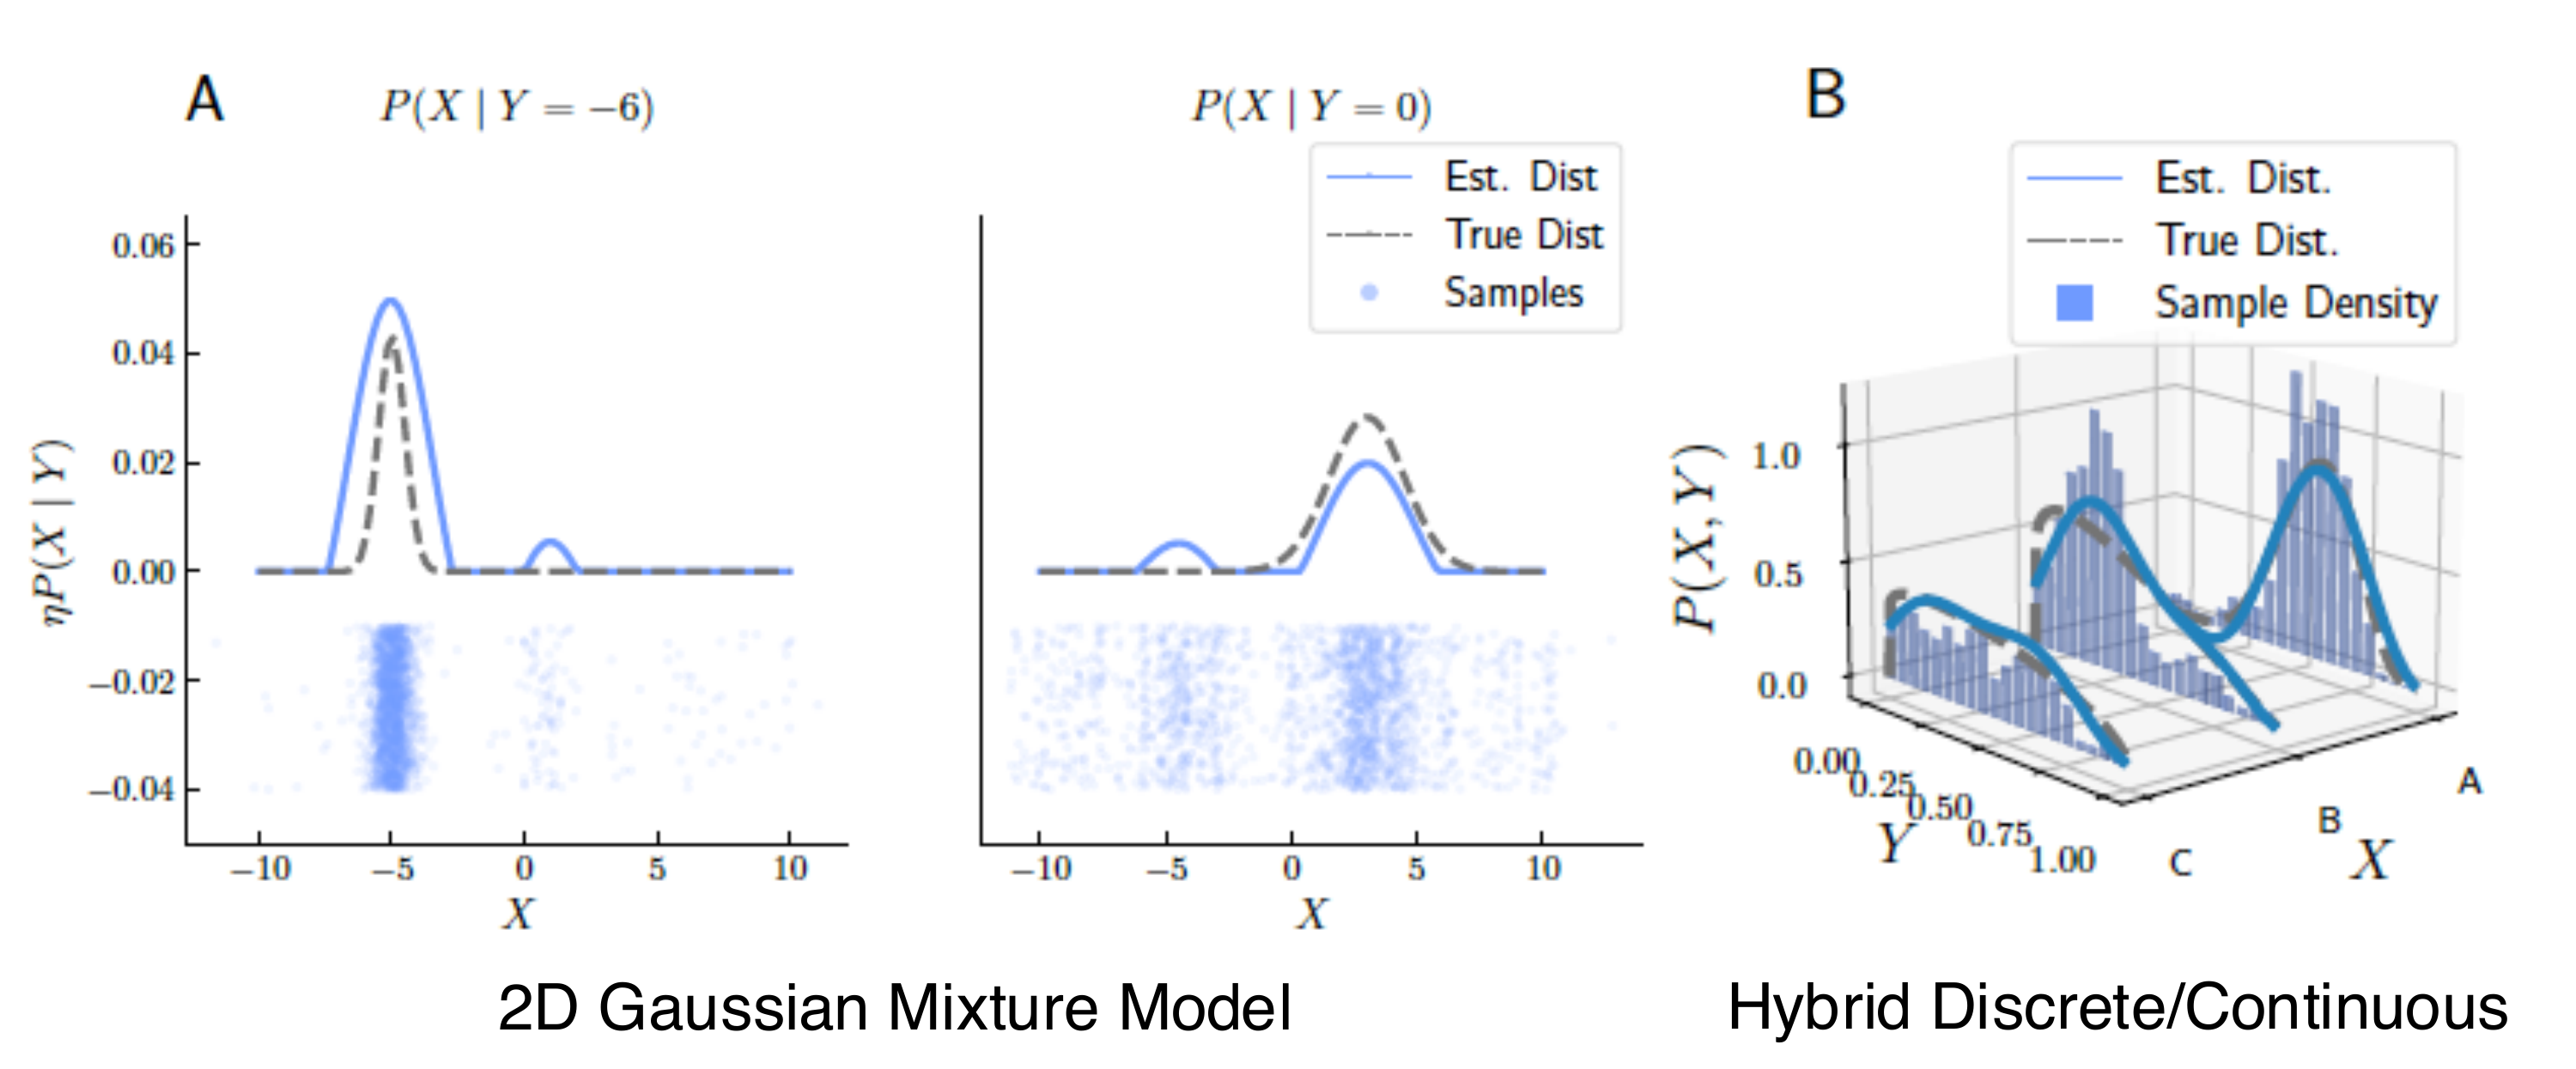
\includegraphics[width=\textwidth,height=0.75\textheight,keepaspectratio]{media/ssp/s35_body.png}
	\end{frame}

	\begin{frame}{SSPs as Probabilities}
		Useful properties:
		\begin{itemize}
			\setlength{\itemsep}{0.75cm}
			\item Provide a general and abstract framework for modelling probabilities
			\item Draw a direct connection between \hl{cognitive models} and \hl{probability statements}
			\item Provide network architectures for conditioning, marginalization, entropy, sampling, and mutual information
		\end{itemize}
	\end{frame}

	\begin{frame}{SSPs for Optimization}
		\begin{itemize}
			\item Three difficult optimization problems
		\end{itemize}
		\centering
		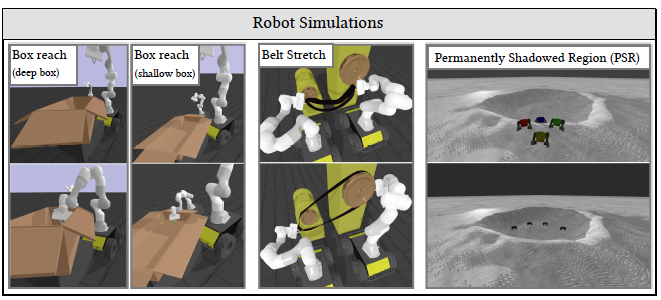
\includegraphics[width=\textwidth,height=0.75\textheight,keepaspectratio]{media/ssp/s36_i1.png}
	\end{frame}

	\begin{frame}{SSPs for Optimization}
		\begin{itemize}
			\item We use SSPs to represent possible trajectories
			\begin{itemize}
				\item Hybrid repn: $\sum (\text{agent} \CC \text{trajectory})$
			\end{itemize}
		\end{itemize}
		\centering
		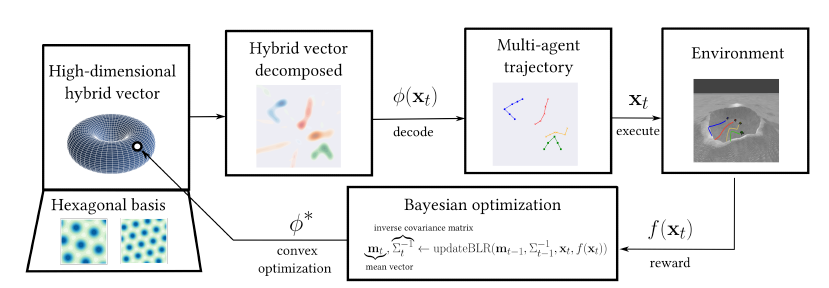
\includegraphics[width=\textwidth,height=0.68\textheight,keepaspectratio]{media/ssp/s37_i1.png}
	\end{frame}

	\begin{frame}{SSPs for Optimization}
		\begin{itemize}
			\item As good or better performance than SoA
		\end{itemize}
		\centering
		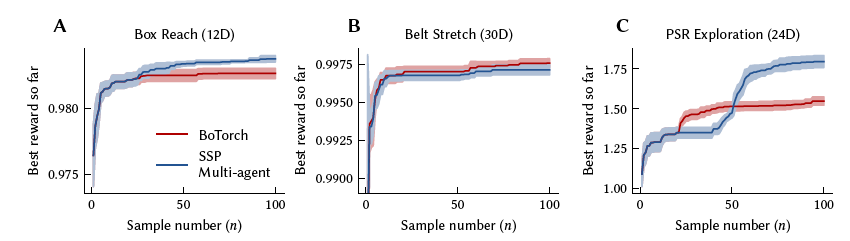
\includegraphics[width=\textwidth,height=0.7\textheight,keepaspectratio]{media/ssp/s38_i1.png}
	\end{frame}

	\begin{frame}{SSPs for Optimization}
		\begin{itemize}
			\item Much faster ($53\times$--$175\times$)
			\begin{itemize}
				\item From $\mathcal{O}(N^3)$ to $\mathcal{O}(1)$ in number of samples
			\end{itemize}
		\end{itemize}
		\centering
		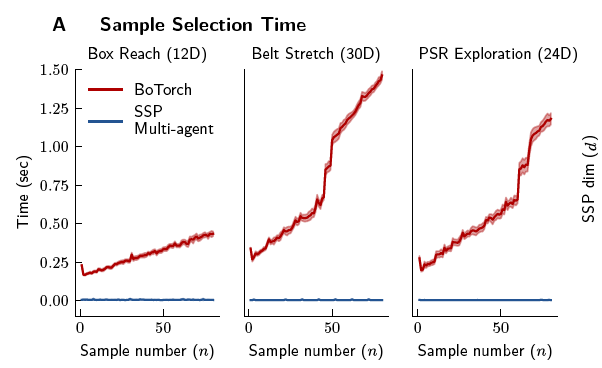
\includegraphics[width=0.85\textwidth,height=0.68\textheight,keepaspectratio]{media/ssp/s39_i1.png}
	\end{frame}

	\begin{frame}{Conclusion}
		\begin{itemize}
			\setlength{\itemsep}{0.5cm}
			\item SSPs support a variety of types of inference for cognitive models
			\item Hybrid spatial and `symbolic' representations
			\item Representations of sampled data that can be used for probabilistic inference
			\item Improves\\[0.25cm]
			\begin{itemize}
				\setlength{\itemsep}{0.25cm}
				\item Interpretability
				\item Efficiency (SWaP critical)
			\end{itemize}
			\item Best engineered systems continue to learn from understanding biological solutions
		\end{itemize}
	\end{frame}

	\backupbegin

	\begin{frame}[noframenumbering]{Image sources}
		\small
		\textbf{Title slide}\\Cover art from \enquote{How to Build a Brain} (Eliasmith, 2013).\\[0.25cm]
		\textbf{Empirical Grid Cells}\\Grid cell recordings adapted from Moser et al.\ (2015).
	\end{frame}

	\backupend

\end{document}
